\documentclass[letterpaper]{article} % DO NOT CHANGE THIS
\usepackage{aaai24}  % DO NOT CHANGE THIS
\usepackage{times}  % DO NOT CHANGE THIS
\usepackage{helvet}  % DO NOT CHANGE THIS
\usepackage{courier}  % DO NOT CHANGE THIS
\usepackage[hyphens]{url}  % DO NOT CHANGE THIS
\usepackage{graphicx} % DO NOT CHANGE THIS
\urlstyle{rm} % DO NOT CHANGE THIS
\def\UrlFont{\rm}  % DO NOT CHANGE THIS
\usepackage{natbib}  % DO NOT CHANGE THIS AND DO NOT ADD ANY OPTIONS TO IT
\usepackage{caption} % DO NOT CHANGE THIS AND DO NOT ADD ANY OPTIONS TO IT
\frenchspacing  % DO NOT CHANGE THIS
\setlength{\pdfpagewidth}{8.5in}  % DO NOT CHANGE THIS
\setlength{\pdfpageheight}{11in}  % DO NOT CHANGE THIS
\usepackage{algorithm}
\usepackage{algorithmic}

\usepackage{tabularx}
\usepackage{amsmath}
\usepackage{amssymb}
\usepackage{graphicx}
\usepackage{booktabs}
\usepackage{threeparttable} \usepackage{multirow}

\usepackage{subfigure}

\newtheorem{theorem}{Theorem}
\newtheorem{proposition}{Proposition}
\newtheorem{lemma}{Lemma}
\newtheorem{fact}{Fact}
\newtheorem{prop}{Proposition}
\newtheorem{corollary}{Corollary}
\newtheorem{definition}{Definition}
\newtheorem{assumption}{Assumption}
\newtheorem{remark}{Remark}

\usepackage{newfloat}
\usepackage{listings}
\DeclareCaptionStyle{ruled}{labelfont=normalfont,labelsep=colon,strut=off} % DO NOT CHANGE THIS
\lstset{%
basicstyle={\footnotesize\ttfamily},% footnotesize acceptable for monospace
numbers=left,numberstyle=\footnotesize,xleftmargin=2em,% show line numbers, remove this entire line if you don't want the numbers.
aboveskip=0pt,belowskip=0pt,%
showstringspaces=false,tabsize=2,breaklines=true}
\floatstyle{ruled}
\newfloat{listing}{tb}{lst}{}
\floatname{listing}{Listing}


\setcounter{secnumdepth}{0} %May be changed to 1 or 2 if section numbers are desired.



\title{Provably Convergent Federated Trilevel Learning}
\author {
Yang Jiao\textsuperscript{\rm 1},
Kai Yang\textsuperscript{\rm 1,2,3}\thanks{Corresponding author (e-mail: kaiyang@tongji.edu.cn).},
Tiancheng Wu\textsuperscript{\rm 1},
Chengtao Jian\textsuperscript{\rm 1},
Jianwei Huang\textsuperscript{\rm 4,5}
}
\affiliations {
\textsuperscript{\rm 1}Department of Computer Science and Technology, Tongji University\\
\textsuperscript{\rm 2} Key Laboratory of Embedded System and Service Computing Ministry of Education at Tongji University\\
\textsuperscript{\rm 3}Shanghai Research Institute for Intelligent Autonomous Systems \\
\textsuperscript{\rm 4}School of Science and Engineering, The Chinese University of Hong Kong, Shenzhen\\
\textsuperscript{\rm 5}Shenzhen Institute of Artificial Intelligence and Robotics for Society\\

yangjiao@tongji.edu.cn, kaiyang@tongji.edu.cn, tony318@tongji.edu.cn, jct@tongji.edu.cn, \\
jianweihuang@cuhk.edu.cn
}


\iffalse
\author{
Written by AAAI Press Staff\textsuperscript{\rm 1}\thanks{With help from the AAAI Publications Committee.}\\
AAAI Style Contributions by Pater Patel Schneider,
Sunil Issar,\\
J. Scott Penberthy,
George Ferguson,
Hans Guesgen,
Francisco Cruz\equalcontrib,
Marc Pujol-Gonzalez\equalcontrib
}
\affiliations{
\textsuperscript{\rm 1}Association for the Advancement of Artificial Intelligence\\


1900 Embarcadero Road, Suite 101\\
Palo Alto, California 94303-3310 USA\\
proceedings-questions@aaai.org
}
\fi


\iffalse
\title{My Publication Title --- Single Author}
\author {
Author Name
}
\affiliations{
Affiliation\\
Affiliation Line 2\\
name@example.com
}
\fi


\usepackage{bibentry}

\begin{document}

\maketitle

\begin{abstract}
Trilevel learning, also called trilevel optimization (TLO), has been recognized as a powerful modelling tool for hierarchical decision process and widely applied in many machine learning applications, such as robust neural architecture search, hyperparameter optimization, and domain adaptation. Tackling TLO problems has presented a great challenge due to their nested decision-making structure. In addition, existing works on TLO face the following key challenges: 1) they all focus on the non-distributed setting, which may lead to privacy breach; 2) they do not offer any non-asymptotic convergence analysis which characterizes how fast an algorithm converges. To address the aforementioned challenges, this paper proposes an asynchronous federated trilevel optimization method to solve TLO problems. The proposed method utilizes $\mu$-cuts to construct a hyper-polyhedral approximation for the TLO problem and solve it in an asynchronous manner. We demonstrate that the proposed $\mu$-cuts are applicable to not only convex functions but also a wide range of non-convex functions that meet the $\mu$-weakly convex assumption. Furthermore, we theoretically analyze the non-asymptotic convergence rate for the proposed method by showing its iteration complexity to obtain $\epsilon$-stationary point is upper bounded by $\mathcal{O}(\frac{1}{\epsilon^2})$. Extensive experiments on real-world datasets have been conducted to elucidate the superiority of the proposed method, e.g., it has a  faster convergence rate with a maximum acceleration of approximately 80$\%$.

\end{abstract}

\section{Introduction}

Recently, trilevel learning, also called trilevel optimization (TLO), has found applications in many machine learning tasks, e.g., robust neural architecture search \cite{guo2020meets}, robust hyperparameter optimization \cite{sato2021gradient} and domain adaptation \cite{raghu2021meta}. Trilevel optimization problems refer to the optimization problems that involve three-level optimization problems and thus have a trilevel hierarchy \cite{avraamidou2018mixed,sato2021gradient}. A general form of trilevel optimization problem is given by,
\begin{equation}
\label{eq:trilevel}
\begin{array}{l}
\min  {{f_{1}}({\boldsymbol{x}_1},{\boldsymbol{x}_2},{\boldsymbol{x}_3})} \;{\rm{s}}.{\rm{t}}. \%removedVspace
\qquad {\boldsymbol{x}_2} = \mathop {\arg \min }\limits_{{\boldsymbol{x}_2}'}  {{f_{2}}({\boldsymbol{x}_1},{\boldsymbol{x}_2}',{\boldsymbol{x}_3})} \;{\rm{s}}.{\rm{t}}. \\
\qquad \qquad {\boldsymbol{x}_3} = \mathop {\arg \min }\limits_{{\boldsymbol{x}_3}'}  {{f_{3}}({\boldsymbol{x}_1},{\boldsymbol{x}_2}',{\boldsymbol{x}_3}')} \\
{\mathop{\rm var}}. \qquad \qquad {\boldsymbol{x}_1},{\boldsymbol{x}_2},{\boldsymbol{x}_3},
\end{array}
\end{equation}
where $f_1, f_2, f_3$ respectively denote the first, second, and third level objectives. Here $\boldsymbol{x}_1 \!\in\! \mathbb{R}^{d_1}, \boldsymbol{x}_2 \!\in\! \mathbb{R}^{d_2}, \boldsymbol{x}_3 \!\in\! \mathbb{R}^{d_3}$ are variables. Despite its wide applications, the development of solution methods was predominately limited
to bilevel optimization (BLO) \cite{ji2021bilevel,franceschi2018bilevel} primarily due to the escalated difficulty in solving the TLO problem \cite{sato2021gradient}. The literature, specifically \cite{blair1992computational,avraamidou2018mixed}, highlights that the complexity associated with solving problems characterized by hierarchical structures comprising more than two levels is substantially greater compared to that of bilevel optimization problems.

Theoretical work on solving TLO problems only emerge during the recent several years. A hypergradient (gradient)-based method is proposed in \cite{sato2021gradient}, which uses $K$ gradient descent steps to replace the lower-level problem to solve the TLO problems. This algorithm in \cite{sato2021gradient} is one of the first results that establish theoretical guarantees for solving the TLO problem.  A general automatic differentiation technique is proposed in \cite{choe2022betty}, which is based on the interpretation of TLO as a special type of dataflow graph.
Nevertheless, there are still some issues that have not been addressed in the prior work, including 1) in TLO applications, data may be acquired and disseminated across multiple nodes, the prior works only solve the TLO problems in a non-distributed manner, which needs to collect a massive amount of data to a single server and may lead to the data privacy risks  \cite{subramanya2021centralized,jiao2022asynchronous,han2020adaptive}. Moreover, the synchronous federated algorithms often suffer from straggler
problems and will immediately stop working if some workers fail to communicate \cite{jiao2022asynchronous}. Therefore, developing asynchronous federated algorithms for TLO is significantly important. 2) The existing TLO works only provide the asymptotic convergence guarantee for their algorithms. In order to understand the convergence speed of the proposed algorithm, non-asymptotic convergence analysis that can characterize how fast an algorithm converges in practice is required.

To this end, we propose an \textbf{A}synchronous \textbf{F}ederated \textbf{T}rilevel \textbf{O}ptimization method (AFTO) in this paper. The proposed AFTO can effectively solve the TLO problems in an asynchronous federated manner. Specifically, it treats the lower-level optimization problem as a constraint to the upper-level and utilizes $\mu$-cuts to construct the hyper-polyhedral approximation, then an effective asynchronous algorithm is developed.  In the context of trilevel learning problems, the objective functions at each level are usually non-convex, thus the cutting plane methods tailored for convex functions \cite{jiao2022asynchronous,franc2011cutting} are found to be inapplicable. To our best knowledge, the proposed methodology referred to as  $\mu$-cut represents the first approach that is capable of constructing cutting planes for trilevel learning problems characterized by non-convex objectives. Furthermore, we demonstrate that the proposed method is guaranteed to converge and theoretically analyze the non-asymptotic convergence rate in terms of iteration complexity.


The contributions of this work are summarized as follows.

\textbf{1.} An asynchronous federated trilevel optimization method is proposed in this work for trilevel learning. To our best knowledge, it is the first work designing algorithms to solve the trilevel learning problem in an asynchronous distributed manner.


\textbf{2.} A novel hyper-polyhedral approximation method via  $\mu$-cut is proposed in this work. The proposed $\mu$-cut can be applied to trilevel learning with non-convex objectives. We further demonstrate that the iteration complexity of the proposed method to achieve the $\epsilon$-stationary point is upper bounded by $\mathcal{O}(\frac{1}{\epsilon^2})$.


\textbf{3.} Extensive experiments on real-world datasets justify the superiority of the proposed method and underscore the significant benefits of employing the hyper-polyhedral approximation for trilevel learning.

\section{Related Work}
\subsection{Trilevel Optimization}
Trilevel optimization has many applications ranging from economics to machine learning. A robust neural architecture search approach is proposed in \cite{guo2020meets}, which integrates the adversarial training into one-shot neural architecture search and can be regarded as solving a trilevel optimization problem. TimeAutoAD \cite{jiao2022timeautoad} is proposed to automatically configure the anomaly detection pipeline and optimize the hyperparameters for multivariate time series anomaly detection. The optimization problem that TimeAutoAD aims to solve can be viewed as a trilevel optimization problem. And a method is proposed in \cite{raghu2021meta} to solve the trilevel optimization problem which involves hyperparameter optimization and two-level pretraining and finetuning. LFM \cite{garg2022learning} is proposed to solve a trilevel optimization problem which consists of data reweight, architecture search, and model training. A general automatic differentiation technique Betty is proposed in \cite{choe2022betty}, which can be utilized to solve the trilevel optimization problem. However, the aforementioned algorithms do not provide any convergence guarantee. A hypergradient-based algorithm with asymptotic convergence guarantee is proposed in \cite{sato2021gradient}, which can be employed in trilevel optimization problems. Nevertheless, the existing works focus on solving the TLO problems in a non-distributed manner and do not provide any non-asymptotic convergence analysis. Instead, an efficient asynchronous algorithm with non-asymptotic convergence guarantee is proposed in this work for solving TLO problems. To our best knowledge, this is the first work that solves TLO problems in an asynchronous federated manner.


\subsection{Polyhedral Approximation}
Polyhedral approximation is a widely-used approximation method \cite{bertsekas2015convex}. The idea behind polyhedral approximation is to approximate either the feasible region or the
epigraph of the objective function of an optimization problem by a set of cutting planes, and the approximation will be gradually refined by adding additional cutting planes. Since the approximate problem is polyhedral, it is usually much easier to solve than the original problem. Following \cite{bertsekas2015convex}, the polyhedral approximation can be broadly divided into two main approaches: outer linearization and inner linearization. The outer linearization \cite{tawarmalani2005polyhedral,yang2008distributed,burger2013polyhedral} (also called cutting plane method) utilizes a set of cutting planes to approximate the feasible region or the
epigraph of the objective function from
without. In contrast, inner linearization \cite{bertsekas2011unifying,trombettoni2011inner} utilizes the convex hulls
of finite numbers of halflines or points to approximate the feasible region or the
epigraph of the objective function from within. Polyhedral approximation has been widely used in convex optimization. A polyhedral approximation method is proposed in \cite{bertsekas2015convex} for convex optimization, which utilizes cutting planes to approximate the original convex optimization problem. In \cite{burger2013polyhedral}, a fully distributed
algorithm is proposed, which is based on an outer polyhedral approximation of
the constraint sets, for the convex and robust distributed optimization
problems in peer-to-peer networks.  In this work, a novel hyper-polyhedral approximation method via $\mu$-cut is proposed for TLO. The proposed $\mu$-cut can be utilized for $\mu$-weakly convex optimization and thus has broader applicability compared with the cutting plane methods for convex optimization.


\section{Asynchronous Federated Trilevel Learning}
Traditional trilevel optimization methods require collecting a massive amount of data to a single server for model training, which may lead to data privacy risks. Solving trilevel optimization problems in a distributed manner is challenging since the trilevel optimization problem is highly-nested which hinders the development of the distributed algorithms.
The distributed trilevel optimization problem can be expressed as,
\begin{equation}
\label{eq:1}
\begin{array}{l}
\min \sum\nolimits_{j = 1}^N {{f_{1,j}}({\boldsymbol{x}_1},{\boldsymbol{x}_2},{\boldsymbol{x}_3})} \;{\rm{s}}.{\rm{t}}. \%removedVspace
\qquad {\boldsymbol{x}_2} = \mathop {\arg \min }\limits_{{\boldsymbol{x}_2}'} \sum\nolimits_{j = 1}^N {{f_{2,j}}({\boldsymbol{x}_1},{\boldsymbol{x}_2}',{\boldsymbol{x}_3})} \;{\rm{s}}.{\rm{t}}. \\
\qquad \qquad {\boldsymbol{x}_3} = \mathop {\arg \min }\limits_{{\boldsymbol{x}_3}'} \sum\nolimits_{j = 1}^N {{f_{3,j}}({\boldsymbol{x}_1},{\boldsymbol{x}_2}',{\boldsymbol{x}_3}')} \%removedVspace
{\mathop{\rm var}}. \qquad \qquad {\boldsymbol{x}_1},{\boldsymbol{x}_2},{\boldsymbol{x}_3},
\end{array}
\end{equation}
where $N$ denotes the number of workers in distributed systems, $f_{1,j}, f_{2,j}, f_{3,j}$ denote the local first, second, and third level objectives in worker $j$, respectively. The problem in Eq. (\ref{eq:1}) can be reformulated as a consensus problem \cite{zhang2014asynchronous,jiao2022distributed},
\begin{equation}
\label{eq:2}
\begin{array}{l}
\min \sum\nolimits_{j} {{f_{1,j}}({\boldsymbol{x}_{1,j}},{\boldsymbol{x}_{2,j}},{\boldsymbol{x}_{3,j}})} \;{\rm{s}}.{\rm{t}}. \\

{\boldsymbol{x}_{1,j}} = {\boldsymbol{z}_1},j = 1, \cdots ,N \\

\! \{{\boldsymbol{x}_{2,j}}\} ,{\boldsymbol{z}_2} \!=\! \mathop {\arg \min }\limits_{\{ {\boldsymbol{x}_{2,j}}'\} ,{\boldsymbol{z}_2}'} \sum\nolimits_{j} {{f_{2,j}}({\boldsymbol{z}_1},{\boldsymbol{x}_{2,j}}',{\boldsymbol{x}_{3,j}})} \;{\rm{s}}.{\rm{t}}. \\

\qquad \quad \;\;\, \,  {\boldsymbol{x}_{2,j}}' = {\boldsymbol{z}_2}',j = 1, \cdots ,N \\

\qquad \quad \;\;\,   \{{\boldsymbol{x}_{3,j}}\} ,{\boldsymbol{z}_3} \!=\! \mathop {\arg \min }\limits_{\{{\boldsymbol{x}_{3,j}}'\},{\boldsymbol{z}_3}'} \! \sum\nolimits_{j} \!{{f_{3,j}}({\boldsymbol{z}_1},{\boldsymbol{z}_2}',{\boldsymbol{x}_{3,j}}')} \,{\rm{s}}.{\rm{t}}. \\

\qquad \qquad \qquad \qquad \quad   {\boldsymbol{x}_{3,j}}' = {\boldsymbol{z}_3}',j = 1, \cdots ,N \%removedVspace

{\mathop{\rm var}}. \qquad  \qquad \{{\boldsymbol{x}_{1,j}}\} ,{\rm{\{ }}{\boldsymbol{x}_{2,j}}\} ,{\rm{\{ }}{\boldsymbol{x}_{3,j}}\} ,{\boldsymbol{z}_1}{\rm{,}}{\boldsymbol{z}_2},{\boldsymbol{z}_3},
\end{array}
\end{equation}
where $\boldsymbol{x}_{1,j} \!\in\! \mathbb{R}^{d_1}, \boldsymbol{x}_{2,j}\!\in\! \mathbb{R}^{d_2}, \boldsymbol{x}_{3,j}\!\in\! \mathbb{R}^{d_3}$ denote the local variables in worker $j$, and $\boldsymbol{z}_1 \!\in\! \mathbb{R}^{d_1}, \boldsymbol{z}_2\!\in\! \mathbb{R}^{d_2}, \boldsymbol{z}_3\!\in\! \mathbb{R}^{d_3}$ denote the consensus variables in the master. This reformulation in Eq. (\ref{eq:2}) can facilitate the development of distributed algorithms for trilevel optimization problems based on the parameter-server architecture \cite{assran2020advances}. The remaining procedure of the proposed method can be divided into three steps. First, how to construct the hyper-polyhedral approximation for distributed TLO problems is proposed. Then, an effective asynchronous federated algorithm is developed. Finally, how to update the $\mu$-cuts to refine the hyper-polyhedral approximation is proposed.

\subsection{Hyper-Polyhedral Approximation}
Different from the traditional polyhedral approximation method \cite{bertsekas2015convex,franc2011cutting,burger2013polyhedral}, a novel hyper-polyhedral approximation method is proposed for distributed TLO problems in this work. By utilizing the proposed hyper-polyhedral approximation,
the distributed algorithms can be easier to develop for TLO problems. Specifically, the proposed hyper-polytope consists of the ${\rm{\uppercase\expandafter{\romannumeral1}}}^{\rm{st}}$ layer and ${\rm{\uppercase\expandafter{\romannumeral2}}}^{\rm{nd}}$  layer polytopes, which are introduced as follows.


\subsubsection{${\rm{\uppercase\expandafter{\romannumeral1}}}^{\rm{st}}$ layer Polyhedral Approximation:}

First, defining  $h_{\rm{\uppercase\expandafter{\romannumeral1}}}(\{{\boldsymbol{x}_{3,j}}\},\boldsymbol{z}_1, {\boldsymbol{z}_2}',\boldsymbol{z}_3 ) \!=\!||\left[ \begin{array}{l}
\! \{{\boldsymbol{x}_{3,j}}\} \! \\
\boldsymbol{z}_3
\end{array} \right]  \!-\!\phi_{{\rm{\uppercase\expandafter{\romannumeral1}}}}({\boldsymbol{z}_1},{\boldsymbol{z}_2}')||^2 $ and $\phi_{\rm{\uppercase\expandafter{\romannumeral1}}}({\boldsymbol{z}_1},{\boldsymbol{z}_2}')\!=\! \mathop{\arg \min }\nolimits_{\{{\boldsymbol{x}_{3,j}}'\},{\boldsymbol{z}_3}'}\{ \sum\nolimits_{j=1}^N \! {{f_{3,j}}({\boldsymbol{z}_1},{\boldsymbol{z}_2}',{\boldsymbol{x}_{3,j}}')}: {\boldsymbol{x}_{3,j}}' \!=\! {\boldsymbol{z}_3}',\forall j\}$.  In trilevel optimization, the third level optimization problem can be viewed as the constraint to the second level optimization problem \cite{chen2022trilevel}, i.e., $h_{\rm{\uppercase\expandafter{\romannumeral1}}}(\{{\boldsymbol{x}_{3,j}}\},\boldsymbol{z}_1, {\boldsymbol{z}_2}',\boldsymbol{z}_3 )\!=\!0$.  A consensus problem needs to be solved in a distributed manner if the exact $\phi_{\rm{\uppercase\expandafter{\romannumeral1}}}({\boldsymbol{z}_1},{\boldsymbol{z}_2}')$ is required. In many works in bilevel \cite{ji2021bilevel,liu2021towards,jiao2022asynchronous} and trilevel \cite{sato2021gradient} optimization, the exact $\phi_{\rm{\uppercase\expandafter{\romannumeral1}}}({\boldsymbol{z}_1},{\boldsymbol{z}_2}')$ can be replaced by an estimate of $\phi_{\rm{\uppercase\expandafter{\romannumeral1}}}({\boldsymbol{z}_1},{\boldsymbol{z}_2}')$, and we utilize the results after $K$ communication rounds between the master and workers as the estimate of $\phi_{\rm{\uppercase\expandafter{\romannumeral1}}}({\boldsymbol{z}_1},{\boldsymbol{z}_2}')$ according to \cite{jiao2022asynchronous}. Specifically, for the third level optimization problem, the augmented Lagrangian function can be written as,
\begin{equation}
\begin{array}{l}
\! L_{p,3} \!=\! \sum\nolimits_{j = 1}^N ( {{f_{3,j}}({\boldsymbol{z}_1},{\boldsymbol{z}_2}'\!,{\boldsymbol{x}_{3,j}}')} + {\boldsymbol{\varphi}_{3,j}^{\top}}({\boldsymbol{x}_{3,j}}'- {\boldsymbol{z}_3}') \%removedVspace
\qquad \qquad \quad \, + \frac{\kappa_3}{2}||{\boldsymbol{x}_{3,j}}'- {\boldsymbol{z}_3}'||^2 ),
\end{array}
\end{equation}
where $L_{p,3} = L_{p,3}({\boldsymbol{z}_1},\!{\boldsymbol{z}_2}'\!, {\boldsymbol{z}_3}'\!,\! \{{\boldsymbol{x}_{3,j}}'\},\! \{\boldsymbol{\varphi}_{3,j}\})$, $\boldsymbol{\varphi}_{3,j} \!\in\! \mathbb{R}^{d_3}$ is the dual variable, and constant $\kappa_3\!>\!0$ is a penalty parameter. In $(k+1)^{\rm{th}}$ communication round, we have that,

\noindent 1) Workers update the local variables,
\begin{equation}
{\boldsymbol{x}_{3,j}^{k+1}}' \!=\! {\boldsymbol{x}_{3,j}^{k}}'\!-\!\eta_{\boldsymbol{x}} \!\nabla_{\boldsymbol{x}_{3,j}} L_{p,3}({\boldsymbol{z}_1},{\boldsymbol{z}_2}'\!, {\boldsymbol{z}_3^k}',\! \{{\boldsymbol{x}_{3,j}^k}'\},\! \{\boldsymbol{\varphi}_{3,j}^k\}),
\end{equation}
where $\eta_{\boldsymbol{x}}$ represents the step-size. Then, workers transmit the local variables ${\boldsymbol{x}_{3,j}^{k+1}}'$ to the master.

\noindent 2) Master updates the variables as follows,
\begin{equation}
{\boldsymbol{z}_3^{k+1}}' \!=\! {\boldsymbol{z}_3^k}' \!-\! \eta_{\boldsymbol{z}}\! \nabla_{\boldsymbol{z}_3} L_{p,3}({\boldsymbol{z}_1},{\boldsymbol{z}_2}' \!, {\boldsymbol{z}_3^k}', \! \{{\boldsymbol{x}_{3,j}^k}'\}, \! \{\boldsymbol{\varphi}_{3,j}^k\}),
\end{equation}
\begin{equation}
\boldsymbol{\varphi}_{3,j}^{k+1} \!=\! \boldsymbol{\varphi}_{3,j}^{k}+\eta_{\boldsymbol{\varphi}}\! \nabla_{\boldsymbol{\varphi}_{3,j}} L_{p,3}({\boldsymbol{z}_1},{\boldsymbol{z}_2}' \!, {\boldsymbol{z}_3^{k+1}}', \! \{{\boldsymbol{x}_{3,j}^{k+1}}'\}, \! \{\boldsymbol{\varphi}_{3,j}^k\}),
\end{equation}
where $\eta_{\boldsymbol{z}}$ and $\eta_{\boldsymbol{\varphi}}$ represent the step-sizes. Then, master broadcasts the ${\boldsymbol{z}_3^{k+1}}'$ and $\boldsymbol{\varphi}_{3,j}^{k+1}$ to workers.


The results after $K$ communication rounds are utilized as the estimate of $\phi_{\rm{\uppercase\expandafter{\romannumeral1}}}({\boldsymbol{z}_1},{\boldsymbol{z}_2}')$, that is,
\begin{equation}
\begin{array}{l}
\label{4_17_12}
\phi_{\rm{\uppercase\expandafter{\romannumeral1}}}({\boldsymbol{z}_1},{\boldsymbol{z}_2}')
\! = \left[ \begin{array}{l}
\! \{ {\boldsymbol{x}_{3,j}^{0}}' \!-\!\sum\nolimits_{k = 0}^{K-1} \! \eta_{\boldsymbol{x}} \! \nabla_{\boldsymbol{x}_{3,j}} L_{p,3}^k \} \! \\%removedVspace

{\boldsymbol{z}_3^{0}}'-\sum\nolimits_{k = 0}^{K-1}\eta_{\boldsymbol{z}} \nabla_{\boldsymbol{z}_3} L_{p,3}^k
\end{array} \right] ,
\end{array}
\end{equation}
where $L_{p,3}^k = L_{p,3}({\boldsymbol{z}_1},{\boldsymbol{z}_2}', {\boldsymbol{z}_3^k}', \{{\boldsymbol{x}_{3,j}^k}'\}, \{\boldsymbol{\varphi}_{3,j}^k\})$. Based on Eq. (\ref{4_17_12}) and the definition of $h_{\rm{\uppercase\expandafter{\romannumeral1}}}$, we have that,
\begin{equation}
\begin{array}{l}
\label{eq:5_8_9}
\!h_{\rm{\uppercase\expandafter{\romannumeral1}}}(\{{\boldsymbol{x}_{3,j}}\},\boldsymbol{z}_1, {\boldsymbol{z}_2}',\boldsymbol{z}_3 ) \\ \!=\! ||\! \left[ \! \begin{array}{l}
\! \{ \boldsymbol{x}_{3,j} - {\boldsymbol{x}_{3,j}^{0}}'+\sum\nolimits_{k = 0}^{K-1} \!
\eta_{\boldsymbol{x}} \nabla_{\boldsymbol{x}_{3,j}} L_{p,3}^k \} \!  \%removedVspace

\boldsymbol{z}_3 - {\boldsymbol{z}_3^{0}}'+\sum\nolimits_{k = 0}^{K-1}\eta_{\boldsymbol{z}} \nabla_{\boldsymbol{z}_3} L_{p,3}^k
\end{array} \! \right] \! ||^2 .
\end{array}
\end{equation}

Inspired by polyhedral approximation method \cite{bertsekas2015convex,burger2013polyhedral}, the \textbf{${\rm{\uppercase\expandafter{\romannumeral1}}}^{\rm{st}}$ layer} \textbf{polytope}, which forms of a set of cutting planes (i.e., linear inequalities), is utilized to approximate the feasible region with respect to the constraint $h_{\rm{\uppercase\expandafter{\romannumeral1}}}(\{{\boldsymbol{x}_{3,j}}\},\boldsymbol{z}_1, {\boldsymbol{z}_2}',\boldsymbol{z}_3 )\! \le \! \varepsilon_{\rm{\uppercase\expandafter{\romannumeral1}}}$, which is a relaxed form of constraint $h_{\rm{\uppercase\expandafter{\romannumeral1}}}(\{{\boldsymbol{x}_{3,j}}\},\boldsymbol{z}_1, {\boldsymbol{z}_2}',\boldsymbol{z}_3 )\!=\!0$ in Eq. (\ref{eq:5_8_9}), and $\varepsilon_{\rm{\uppercase\expandafter{\romannumeral1}}}\!>\!0$  is a pre-set constant. Specifically, the ${\rm{\uppercase\expandafter{\romannumeral1}}}^{\rm{st}}$ layer polytope in $(t+1)^{\rm{th}}$ iteration can be expressed as $P_{\rm{\uppercase\expandafter{\romannumeral1}}}^{t}\!=\!\{{\boldsymbol{a}_{1,l}^{\rm{\uppercase\expandafter{\romannumeral1}}}}^{\top}\!{\boldsymbol{z}_1} + {\boldsymbol{a}_{2,l}^{\rm{\uppercase\expandafter{\romannumeral1}}}}^{\top}\!{\boldsymbol{z}_2}' + {\boldsymbol{a}_{3,l}^{\rm{\uppercase\expandafter{\romannumeral1}}}}^{\top}\!{\boldsymbol{z}_3} + \sum\nolimits_{j = 1}^N {\boldsymbol{b}{{_{j,l}^{\rm{\uppercase\expandafter{\romannumeral1}}}}}}^{\top}\!{\boldsymbol{x}_{3,j}}  \!\le\! c_l^{\rm{\uppercase\expandafter{\romannumeral1}}},l \!=\! 1,\! \cdots\! ,|P_{\rm{\uppercase\expandafter{\romannumeral1}}}^{t}| \}$, where $|P_{\rm{\uppercase\expandafter{\romannumeral1}}}^{t}|$ denotes the number of cutting planes in ${\rm{\uppercase\expandafter{\romannumeral1}}}^{\rm{st}}$ layer polytope and ${\boldsymbol{a}_{i,l}^{\rm{\uppercase\expandafter{\romannumeral1}}}}, {\boldsymbol{b}_{j,l}^{\rm{\uppercase\expandafter{\romannumeral1}}}}, {c_{l}^{\rm{\uppercase\expandafter{\romannumeral1}}}}$ are parameters in $l^{\rm{th}}$ cutting plane (${\rm{\uppercase\expandafter{\romannumeral1}}}^{\rm{st}}$ layer $\mu$-cut). Defining $\hat{h}_{{\rm{\uppercase\expandafter{\romannumeral1}}},l}(\{{\boldsymbol{x}_{3,j}}\},\boldsymbol{z}_1, {\boldsymbol{z}_2}',\boldsymbol{z}_3 ) = {\boldsymbol{a}_{1,l}^{\rm{\uppercase\expandafter{\romannumeral1}}}}^{\top}\!{\boldsymbol{z}_1} + {\boldsymbol{a}_{2,l}^{\rm{\uppercase\expandafter{\romannumeral1}}}}^{\top}\!{\boldsymbol{z}_2}' + {\boldsymbol{a}_{3,l}^{\rm{\uppercase\expandafter{\romannumeral1}}}}^{\top}\!{\boldsymbol{z}_3} + \sum\nolimits_{j = 1}^N {\boldsymbol{b}{{_{j,l}^{\rm{\uppercase\expandafter{\romannumeral1}}}}}}^{\top}\!{\boldsymbol{x}_{3,j}} $, the resulting (bilevel) problem can be expressed as,
\begin{equation}
\label{eq:4}
\begin{array}{l}
\min \sum\nolimits_{j = 1}^N {{f_{1,j}}({\boldsymbol{x}_{1,j}},{\boldsymbol{x}_{2,j}},{\boldsymbol{x}_{3,j}})} \;{\rm{s}}.{\rm{t}}. \\

{\boldsymbol{x}_{1,j}} = {\boldsymbol{z}_1},j = 1, \cdots ,N \\

\{ {\boldsymbol{x}_{2,j}}\} ,{\boldsymbol{z}_2} \!=\! \mathop {\arg \min }\limits_{\{ {\boldsymbol{x}_{2,j}}'\} ,{\boldsymbol{z}_2}'} \sum\nolimits_{j = 1}^N {{f_{2,j}}({\boldsymbol{z}_1},{\boldsymbol{x}_{2,j}}',{\boldsymbol{x}_{3,j}})} \;{\rm{s}}.{\rm{t}}. \\

\qquad \qquad \quad   {\boldsymbol{x}_{2,j}}' = {\boldsymbol{z}_2}',j = 1, \cdots ,N \\

\qquad \qquad \quad   \hat{h}_{{\rm{\uppercase\expandafter{\romannumeral1}}},l}(\{{\boldsymbol{x}_{3,j}}\},\boldsymbol{z}_1, {\boldsymbol{z}_2}',\boldsymbol{z}_3 )  \!\le\! c_l^{\rm{\uppercase\expandafter{\romannumeral1}}},l \!=\! 1,\! \cdots\! ,|P_{\rm{\uppercase\expandafter{\romannumeral1}}}^{t}|\%removedVspace

{\mathop{\rm var}}. \qquad  \quad \{{\boldsymbol{x}_{1,j}}\} ,{\rm{\{ }}{\boldsymbol{x}_{2,j}}\} ,{\rm{\{ }}{\boldsymbol{x}_{3,j}}\} ,{\boldsymbol{z}_1}{\rm{,}}{\boldsymbol{z}_2},{\boldsymbol{z}_3}.
\end{array}
\end{equation}


\subsubsection{${\rm{\uppercase\expandafter{\romannumeral2}}}^{\rm{nd}}$ layer Polyhedral Approximation:}
Defining function $h_{{\rm{\uppercase\expandafter{\romannumeral2}}}}(\{{\boldsymbol{x}_{2,j}}\} ,\{ {\boldsymbol{x}_{3,j}}\} ,{\boldsymbol{z}_1},{\boldsymbol{z}_2},{\boldsymbol{z}_3}) \!= \!||\left[ \begin{array}{l}
\!\{{\boldsymbol{x}_{2,j}}\} \\
\boldsymbol{z}_2
\end{array} \right]  -\phi_{{\rm{\uppercase\expandafter{\romannumeral2}}}}({\boldsymbol{z}_1}, {\boldsymbol{z}_3}, \{{\boldsymbol{x}_{3,j}}\})||^2 $, where $\phi_{{\rm{\uppercase\expandafter{\romannumeral2}}}}({\boldsymbol{z}_1}, {\boldsymbol{z}_3}, \{{\boldsymbol{x}_{3,j}}\})\!=\! \mathop {\arg \min }\nolimits_{\{ {\boldsymbol{x}_{2,j}}'\} ,{\boldsymbol{z}_2}'} \{ \sum\nolimits_{j = 1}^N {{f_{2,j}}({\boldsymbol{z}_1},{\boldsymbol{x}_{2,j}}',{\boldsymbol{x}_{3,j}})}\!:\! {\boldsymbol{x}_{2,j}}' \!=\! {\boldsymbol{z}_2}', \forall j,  {\boldsymbol{a}_{1,l}^{\rm{\uppercase\expandafter{\romannumeral1}}}}^{\top}\!{\boldsymbol{z}_1} + {\boldsymbol{a}_{2,l}^{\rm{\uppercase\expandafter{\romannumeral1}}}}^{\top}\!{\boldsymbol{z}_2}' + {\boldsymbol{a}_{3,l}^{\rm{\uppercase\expandafter{\romannumeral1}}}}^{\top}\!{\boldsymbol{z}_3} + \sum\nolimits_{j = 1}^N {\boldsymbol{b}{{_{j,l}^{\rm{\uppercase\expandafter{\romannumeral1}}}}}}^{\top}\!{\boldsymbol{x}_{3,j}}  \!\le\! c_l^{\rm{\uppercase\expandafter{\romannumeral1}}},\forall l \}$.
In Eq. (\ref{eq:4}), the lower-level optimization problem can be viewed as the constraint to the upper-level optimization problem \cite{sinha2017review,gould2016differentiating}, i.e., $h_{{\rm{\uppercase\expandafter{\romannumeral2}}}}(\{{\boldsymbol{x}_{2,j}}\} ,\{ {\boldsymbol{x}_{3,j}}\} ,{\boldsymbol{z}_1},{\boldsymbol{z}_2},{\boldsymbol{z}_3}) =0$.  Likewise, following \cite{jiao2022asynchronous},  the results after $K$ communication rounds between the master and workers are utilized as the estimate of $\phi_{{\rm{\uppercase\expandafter{\romannumeral2}}}}({\boldsymbol{z}_1}, {\boldsymbol{z}_3}, \{{\boldsymbol{x}_{3,j}}\})$. Specifically, for the lower-level optimization problem in Eq. (\ref{eq:4}), the augmented Lagrangian function is given,
\begin{equation}
\begin{array}{l}
\!   L_{p,2}({\boldsymbol{z}_1},{\boldsymbol{z}_2}', \! \{{\boldsymbol{x}_{2,j}}'\},\! \{ s_l\},\! \{\gamma_l\},\! \{\boldsymbol{\varphi}_{2,j}\}, {\boldsymbol{z}_3},\! \{{\boldsymbol{x}_{3,j}}\}) \\%removedVspace

\!  =  \sum\nolimits_{j=1}^N  ({{f_{2,j}}({\boldsymbol{z}_1},{\boldsymbol{x}_{2,j}}',{\boldsymbol{x}_{3,j}})} \!+\! {\boldsymbol{\varphi}_{2,j}^{\top}}({\boldsymbol{x}_{2,j}}'\! -\! {\boldsymbol{z}_2}')  \\
\! + \frac{\kappa_2}{2}||{\boldsymbol{x}_{2,j}}'\!-\! {\boldsymbol{z}_2}'||^2 )

+\sum\nolimits_{l = 1}^{|P_{\rm{\uppercase\expandafter{\romannumeral1}}}^{t + 1}|} \gamma_l ( \hat{h}_{\rm{\uppercase\expandafter{\romannumeral1}},l}(\{{\boldsymbol{x}_{3,j}}\},\boldsymbol{z}_1, {\boldsymbol{z}_2}',\boldsymbol{z}_3 )
\\
- c_l^{\rm{\uppercase\expandafter{\romannumeral1}}} \!+\!s_l )
\! + \! \sum\nolimits_{l = 1}^{|P_{\rm{\uppercase\expandafter{\romannumeral1}}}^{t + 1}|} \! \frac{\rho_2}{2} || \hat{h}_{{\rm{\uppercase\expandafter{\romannumeral1}}},l}(\{{\boldsymbol{x}_{3,j}}\},\boldsymbol{z}_1, {\boldsymbol{z}_2}',\boldsymbol{z}_3 ) \! - \! c_l^{\rm{\uppercase\expandafter{\romannumeral1}}} \! + \! s_l||^2,
\end{array}
\end{equation}
where $\gamma_l \!\in\! \mathbb{R}^1$, ${\boldsymbol{\varphi}_{2,j}}\!\in\! \mathbb{R}^{d_2}$ are dual variables, $s_l\!\in\!\mathbb{R}^1_{+},\forall l$ are the slack variables introduced in the inequality constraints, constants $\kappa_2\!>\!0$, $\rho_2\!>\!0$ are penalty parameters. The details of each communication round are presented in Appendix B in the supplementary material.  After $K$ communication rounds, we can obtain the estimate of $\phi_{{\rm{\uppercase\expandafter{\romannumeral2}}}}({\boldsymbol{z}_1}, {\boldsymbol{z}_3}, \{{\boldsymbol{x}_{3,j}}\})$ and the corresponding $h_{{\rm{\uppercase\expandafter{\romannumeral2}}}}$ can be expressed as,
\begin{equation}
\label{eq:4_23_18}
\begin{array}{l}
\!    h_{{\rm{\uppercase\expandafter{\romannumeral2}}}}(\{{\boldsymbol{x}_{2,j}}\} ,\{ {\boldsymbol{x}_{3,j}}\} ,{\boldsymbol{z}_1}, {\boldsymbol{z}_2},{\boldsymbol{z}_3}) \\

\!=\! ||\! \left[\! \begin{array}{l}
\! \{ \boldsymbol{x}_{2,j} - {\boldsymbol{x}_{2,j}^{0}}'+\sum\nolimits_{k = 0}^{K-1} \! \eta_{\boldsymbol{x}}  \nabla_{\boldsymbol{x}_{2,j}}  L_{p,2}^k \} \! \\%removedVspace

\boldsymbol{z}_2 - {\boldsymbol{z}_2^{0}}'+\sum\nolimits_{k = 0}^{K-1} \eta_{\boldsymbol{z}} \nabla_{\boldsymbol{z}_2}  L_{p,2}^k
\end{array} \! \right]\!  ||^2 ,
\end{array}
\end{equation}
where $L_{p,2}^k$ is the simplified form of  $ L_{p,2}({\boldsymbol{z}_1},{\boldsymbol{z}_2^k}', \!\{{\boldsymbol{x}_{2,j}^k}'\}, \!\{ s_l^k\},\!\{\gamma_l^k\},\!\{\boldsymbol{\varphi}_{2,j}^k\},\! {\boldsymbol{z}_3}, \!\{{\boldsymbol{x}_{3,j}}\})$. Next, relaxing constraint $h_{{\rm{\uppercase\expandafter{\romannumeral2}}}}(\{{\boldsymbol{x}_{2,j}}\} ,\{ {\boldsymbol{x}_{3,j}}\} ,{\boldsymbol{z}_1},{\boldsymbol{z}_2},{\boldsymbol{z}_3})\!=\!0$ and utilizing \textbf{${\rm{\uppercase\expandafter{\romannumeral2}}}^{\rm{nd}}$ layer} \textbf{polytope} to approximate the feasible region of relaxed constraint $h_{{\rm{\uppercase\expandafter{\romannumeral2}}}}(\{{\boldsymbol{x}_{2,j}}\} ,\{ {\boldsymbol{x}_{3,j}}\} ,{\boldsymbol{z}_1}{\rm{,}}{\boldsymbol{z}_2},{\boldsymbol{z}_3})\!\le\! \varepsilon_{\rm{\uppercase\expandafter{\romannumeral2}}}$. Specifically, the ${\rm{\uppercase\expandafter{\romannumeral2}}}^{\rm{nd}}$ layer polytope can be expressed as $P_{{\rm{\uppercase\expandafter{\romannumeral2}}}}^{t} \!=\! \{\sum\nolimits_{i = 1}^3 {\boldsymbol{a}_{i,l}^{{\rm{\uppercase\expandafter{\romannumeral2}}}}} ^{\top}\!{\boldsymbol{z}_i} + \sum\nolimits_{i = 2}^3 {\sum\nolimits_{j = 1}^N {{\boldsymbol{b}}{{_{i,j,l}^{{\rm{\uppercase\expandafter{\romannumeral2}}}}}}}^{\top}\!{\boldsymbol{x}_{i,j}} }  \!\le\! c_l^{{\rm{\uppercase\expandafter{\romannumeral2}}}},l \!=\! 1,\! \cdots \!,|P_{{\rm{\uppercase\expandafter{\romannumeral2}}}}^{t}|\}$ in $(t+1)^{\rm{th}}$ iteration, where $|P_{{\rm{\uppercase\expandafter{\romannumeral2}}}}^{t}|$ represents the number of cutting planes in $P_{{\rm{\uppercase\expandafter{\romannumeral2}}}}^{t}$, and ${\boldsymbol{a}_{i,l}^{{\rm{\uppercase\expandafter{\romannumeral2}}}}},
{\boldsymbol{b}{{_{i,j,l}^{{\rm{\uppercase\expandafter{\romannumeral2}}}}}}},
c_l^{{\rm{\uppercase\expandafter{\romannumeral2}}}}$ are parameters in $l^{\rm{th}}$ cutting plane (${\rm{\uppercase\expandafter{\romannumeral2}}}^{\rm{nd}}$ layer $\mu$-cut). Thus, the resulting \textbf{hyper-polyhedral} \textbf{approximation} \textbf{problem} is,
\begin{equation}
\label{eq:outer_poly}
\begin{array}{l}
\min \sum\nolimits_{j = 1}^N {{f_{1,j}}({\boldsymbol{x}_{1,j}},{\boldsymbol{x}_{2,j}},{\boldsymbol{x}_{3,j}})} \;{\rm{s}}.{\rm{t}}. \%removedVspace

\; {\boldsymbol{x}_{1,j}} = {\boldsymbol{z}_1},j = 1, \cdots ,N \%removedVspace

\; \sum\nolimits_{i = 1}^3 \! {\boldsymbol{a}_{i,l}^{{\rm{\uppercase\expandafter{\romannumeral2}}}}} ^{\top}\!{\boldsymbol{z}_i} \!+ \!\sum\nolimits_{i = 2}^3 \!{\sum\nolimits_{j = 1}^N \!{\boldsymbol{b}{{_{i,j,l}^{{\rm{\uppercase\expandafter{\romannumeral2}}}}}}}^{\top}\!{\boldsymbol{x}_{i,j}} }  \!\le\! c_l^{{\rm{\uppercase\expandafter{\romannumeral2}}}},l \!=\! 1,\! \cdots \!,|P_{{\rm{\uppercase\expandafter{\romannumeral2}}}}^{t}| \%removedVspace

{\mathop{\rm var}}.\qquad  \{{\boldsymbol{x}_{1,j}}\} ,{\rm{\{ }}{\boldsymbol{x}_{2,j}}\} ,{\rm{\{ }}{\boldsymbol{x}_{3,j}}\} ,{\boldsymbol{z}_1}{\rm{,}}{\boldsymbol{z}_2},{\boldsymbol{z}_3}.
\end{array}
\end{equation}

It is worth mentioning that solving the TLO problem is theoretically NP-hard (even solving the inner bilevel problem in TLO is NP-hard \cite{ben1990computational}). Thus, its unlikely to design a polynomial-time algorithm for the distributed TLO problem unless P = NP \cite{arora2009computational}.  In this work, the hyper-polyhedral
approximation problem in Eq. (\ref{eq:outer_poly}) is a convex relaxation problem of the distributed TLO problem in Eq. (\ref{eq:1}), and the relaxation will be continuously tightened as $\mu$-cuts are added. Detailed discussions are provided in Appendix D.


\subsection{Asynchronous Federated Algorithm}
The synchronous and asynchronous federated algorithms have different application scenarios \cite{su2022gba}. The synchronous algorithm is preferred when the delay of each worker is not much different, and the asynchronous algorithm suits better when there are stragglers in the distributed system. In this work, an asynchronous algorithm is proposed to solve the trilevel optimization problem. Specifically, in the proposed asynchronous algorithm, we set the master
updates its variables once it receives updates from $S (1\le S \le N)$ workers, i.e., active workers, at every iteration, and every
worker has to communicate with the master at least once every $\tau$ iterations to alleviate the staleness issues \cite{zhang2014asynchronous}. It is worth mentioning that $S$ can be flexibly adjusted based on whether there are stragglers, the proposed algorithm becomes synchronous when we set $S=N$, thus the proposed asynchronous algorithm is effective and flexible. First, the Lagrangian function of Eq. (\ref{eq:outer_poly}) can be expressed as,
\begin{equation}
\begin{array}{l}
L_p(\{{\boldsymbol{x}_{1,j}}\} ,\!\{{\boldsymbol{x}_{2,j}}\} ,\!\{{\boldsymbol{x}_{3,j}}\} ,{\boldsymbol{z}_1},{\boldsymbol{z}_2},{\boldsymbol{z}_3},\! \{\lambda_l\}, \!\{\boldsymbol{\theta}_j\} ) \\

= \sum\nolimits_{j = 1}^N \! {{f_{1,j}}({\boldsymbol{x}_{1,j}},{\boldsymbol{x}_{2,j}},{\boldsymbol{x}_{3,j}})} \! +\! \sum\nolimits_{j = 1}^N \!{{\boldsymbol{\theta}_j}}^{\top} ({\boldsymbol{x}_{1,j}}\! -\! {\boldsymbol{z}_1})\\

+ \sum\nolimits_{l = 1}^{|P_{{\rm{\uppercase\expandafter{\romannumeral2}}}}^{t}|} {{\lambda _l}} ({\sum\nolimits_{i = 1}^3 {\boldsymbol{a}_{i,l}^{{\rm{\uppercase\expandafter{\romannumeral2}}}}} ^{\top}}{\boldsymbol{z}_i} \!+\! \sum\nolimits_{i = 2}^3 \! {\sum\nolimits_{j = 1}^N {\boldsymbol{b}{{_{i,j,l}^{{\rm{\uppercase\expandafter{\romannumeral2}}}}}^{\top}}{\boldsymbol{x}_{i,j}}} } \! -\! c_l^{{\rm{\uppercase\expandafter{\romannumeral2}}}}),
\end{array}
\end{equation}
where $\lambda _l\!\in\!\mathbb{R}^1_{+}$, $\boldsymbol{\theta}_j\!\in\!\mathbb{R}^{d_1}$ are dual variables. Following \cite{xu2020unified,jiao2022asynchronous}, the regularized Lagrangian function is used to update variables as follows,
\begin{equation}
\begin{array}{l}
\widehat{L}_p(\{{\boldsymbol{x}_{1,j}}\} ,\!\{{\boldsymbol{x}_{2,j}}\} ,\!\{{\boldsymbol{x}_{3,j}}\} ,{\boldsymbol{z}_1},{\boldsymbol{z}_2},{\boldsymbol{z}_3},\! \{\lambda_l\}, \!\{\boldsymbol{\theta}_j\} ) \\ = {L_p} - \sum\nolimits_{l = 1}^{|P_{{\rm{\uppercase\expandafter{\romannumeral2}}}}^{t}|} \!\frac{c_1^t}{2}||\lambda_l||^2 - \sum\nolimits_{j = 1}^{N}\! \frac{c_2^t}{2}||\boldsymbol{\theta}_j||^2,
\end{array}
\end{equation}
where $L_p\!=\!L_p(\{{\boldsymbol{x}_{1,j}}\} ,\!\{{\boldsymbol{x}_{2,j}}\} ,\!\{{\boldsymbol{x}_{3,j}}\} ,\!{\boldsymbol{z}_1},\!{\boldsymbol{z}_2},\!{\boldsymbol{z}_3},\! \{\lambda_l\}, \!\{\boldsymbol{\theta}_j\} )$, and $c_1^t$, $c_2^t$ are the regularization terms in $(t+1)^{\rm{th}}$ iteration. We set that ${c_1^t} =1/{{{\eta _{{\lambda}}}}{(t+1)^{\frac{1}{4}}}} \ge  \underline{c}_1$, ${c_2^t} = 1/{{{\eta _{{\boldsymbol{\theta }}}}}{(t+1)^{\frac{1}{4}}}}  \ge  \underline{c}_2$ are two nonnegative non-increasing sequences, where $\eta _{{\lambda}}$, $\eta _{{\boldsymbol{\theta }}}$, $\underline{c}_1$, $\underline{c}_2$ are constants, and $\underline{c}_1$, $\underline{c}_2$ meet that $0\!<\!\underline{c}_1\!<\!1/\eta _{{\lambda}}({({{4M\alpha_4}} / {{{{\eta _{\lambda}}}^2}} \!+\! {{4N\alpha_5}}/{{{{\eta _{\boldsymbol{\theta }}}}^2}})}1/\epsilon)^{\frac{1}{2}}$ and $0\!<\!\underline{c}_2\!<\!1/\eta _{{\boldsymbol{\theta }}} ({({{4M\alpha_4}} / {{{{\eta _{\lambda}}}^2}} \!+\! {{4N\alpha_5}}/{{{{\eta _{\boldsymbol{\theta }}}}^2}})}1/\epsilon)^{\frac{1}{2}}$ ($\epsilon$ refers to the tolerance error, and $\alpha_4$, $\alpha_5$ are constants, which will be introduced below). In $(t+1)^{\rm{th}}$ master iteration, $Q^{t+1} $ is utilized to denote the index set of active workers, and the proposed asynchronous algorithm proceeds as follows,


\noindent (1) \emph{Active} \emph{workers} update the local variables as follows,
\begin{equation}
\label{eq:update_x1_asyn}
{\boldsymbol{x}_{i,j}^{t+1}} = \left\{ \begin{array}{l}
{\boldsymbol{x}_{i,j}^{t}} - \eta_{\boldsymbol{x}_i} \nabla_{\!\boldsymbol{x}_{i,j}} \widehat{L}_p^{\hat{t}_j}, j\in Q^{t+1}\\
{\boldsymbol{x}_{i,j}^{t}}, j\notin Q^{t+1}
\end{array} \right., \forall i,
\end{equation}
where $\eta_{\boldsymbol{x}_i} (\forall i=1,2,3)$ denote the step-sizes, $\widehat{L}_p^{\hat{t}_j} = \widehat{L}_p(\{{\boldsymbol{x}_{i,j}^{\hat{t}_j}}\} ,\!\{{\boldsymbol{z}_i^{\hat{t}_j}}\}, \!\{\lambda_l^{\hat{t}_j}\}, \!\{\boldsymbol{\theta}_j^{\hat{t}_j}\} )$ and ${\hat{t}_j}$ denotes the last iteration that worker $j$ is active. Then, active workers (i.e., worker $j, j\in Q^{t+1}$) transmit the updated local variables, i.e., $\boldsymbol{x}_{i,j}^{t+1}, \forall i$ to the master.

\noindent (2) After receiving the updates from workers, the \emph{master} updates the variables as follows,
\begin{equation}
\label{eq:update_z1_asyn}
\!{\boldsymbol{z}_1^{t+1}} \!=\! {\boldsymbol{z}_1^{t}}\!-\!\eta_{\boldsymbol{z}_1}\! \nabla_{\boldsymbol{z}_1}\widehat{L}_p(\{{\boldsymbol{x}_{i,j}^{t+1}}\} ,\!\{{\boldsymbol{z}_i^t} \},\! \{\lambda_l^t\},\! \{\boldsymbol{\theta}_j^t\} ),
\end{equation}
\begin{equation}
\label{eq:update_z2_asyn}
{\boldsymbol{z}_2^{t+1}} \!=\! {\boldsymbol{z}_2^{t}} \!-\!\eta_{\boldsymbol{z}_2}\! \nabla_{\boldsymbol{z}_2}\widehat{L}_p(\{{\boldsymbol{x}_{i,j}^{t+1}}\} ,\!{\boldsymbol{z}_1^{t+1}}\!,{\boldsymbol{z}_2^t},{\boldsymbol{z}_3^t},\! \{\lambda_l^t\},\! \{\boldsymbol{\theta}_j^t\} ),
\end{equation}
\begin{equation}
\label{eq:update_z3_asyn}
{\boldsymbol{z}_3^{t+1}} \!=\! {\boldsymbol{z}_3^{t}}\!-\!\eta_{\boldsymbol{z}_3} \! \nabla_{\boldsymbol{z}_3}\widehat{L}_p(\{{\boldsymbol{x}_{i,j}^{t+1}}\} ,\!{\boldsymbol{z}_1^{t+1}}\!,{\boldsymbol{z}_2^{t+1}}\!,{\boldsymbol{z}_3^t},\! \{\lambda_l^t\},\! \{\boldsymbol{\theta}_j^t\} ),
\end{equation}
\begin{equation}
\label{eq:update_lambda_asyn}
\!{\lambda_l^{t+1}} \!=\! \mathcal{P}_{\Lambda} ( {\lambda_l^{t}}\!+\!\eta_{\lambda}\! \nabla_{\lambda_l}\widehat{L}_p(\{{\boldsymbol{x}_{i,j}^{t+1}}\} ,\!\{{\boldsymbol{z}_i^{t+1}}\},\! \{\lambda_l^t\},\! \{\boldsymbol{\theta}_j^t\} ) ),
\end{equation}
\begin{equation}
\label{eq:update_theta_asyn}
\!{\boldsymbol{\theta}_j^{t+1}} \!=\! \mathcal{P}_{\Theta}({\boldsymbol{\theta}_j^{t}}\!+\!\eta_{\boldsymbol{\theta}}\! \nabla_{\boldsymbol{\theta}_j}\widehat{L}_p(\{{\boldsymbol{x}_{i,j}^{t+1}}\} ,\!\{{\boldsymbol{z}_i^{t+1}}\}, \!\{\lambda_l^{t+1}\}, \!\{\boldsymbol{\theta}_j^t\} )),
\end{equation}
where $\eta_{\boldsymbol{z}_1}, \eta_{\boldsymbol{z}_2}, \eta_{\boldsymbol{z}_3}, \eta_{\lambda}, \eta_{\boldsymbol{\theta}}$ denote the step-sizes, $\mathcal{P}_{\Lambda}$ and $\mathcal{P}_{\Theta}$ represent the projection onto sets ${\Lambda}=\{ \lambda_l|\; 0 \! \le \! \lambda_l \! \le \! \sqrt{\alpha_4}  \}$ and ${\Theta}=\{ \boldsymbol{\theta}_j|\; ||\boldsymbol{\theta}_j||_{\infty}\! \le \! \sqrt{\alpha_5}/d_1 \}$, where $\alpha_4 \!>\!0$ and $\alpha_5 \!>\!0$ are constants. Then, master broadcasts the updated variables, i.e., ${\boldsymbol{z}_1^{t+1}}, {\boldsymbol{z}_2^{t+1}}, {\boldsymbol{z}_3^{t+1}}, \{\lambda_l^{t+1}\}, \boldsymbol{\theta}_j$ to the active worker $j$. Details are summarized in Algorithm \ref{algorithm:asyn}.

\begin{algorithm}[t]
\caption{Asynchronous Federated Trilevel Learning}
\begin{algorithmic}
\STATE {\bfseries Initialization:}  master iteration $t\! =\! 0$, variables $\{{{\boldsymbol{x}}_{1,j}^0}\},$ $ \{{{\boldsymbol{x}}_{2,j}^0}\}, $ $ \{{{\boldsymbol{x}}_{3,j}^0}\}, \boldsymbol{z}_1^0, \boldsymbol{z}_2^0, \boldsymbol{z}_3^0, \{\lambda_l^0\}, \{\boldsymbol{\theta}_j^0\}$.

\REPEAT

\FOR{\emph{active worker}}
\STATE updates variables $\boldsymbol{x}_{1,j}^{t+1}$, $\boldsymbol{x}_{2,j}^{t+1}$ and $\boldsymbol{x}_{3,j}^{t+1}$ by Eq. (\ref{eq:update_x1_asyn});
\ENDFOR

\STATE active workers send updated local variables to master;

\FOR{\emph{master}}
\STATE updates variables $\boldsymbol{z}_1^{t+1}, \boldsymbol{z}_2^{t+1}, \boldsymbol{z}_3^{t+1}, \{\lambda_l^{t+1}\}, \{\boldsymbol{\theta}_j^{t+1}\}$  by Eq. (\ref{eq:update_z1_asyn}), (\ref{eq:update_z2_asyn}), (\ref{eq:update_z3_asyn}), (\ref{eq:update_lambda_asyn}) and (\ref{eq:update_theta_asyn});
\ENDFOR
\STATE master broadcasts updated variables to active workers;


\IF{$(t+1)$ mod $T_{\rm{pre}}$ $==0$ and $t<T_1$}
\STATE   new ${\rm{\uppercase\expandafter{\romannumeral1}}}^{\rm{st}}$ layer $\mu$-cut ${cp_{\rm{\uppercase\expandafter{\romannumeral1}}}}$ is generated by Eq. (\ref{eq:new_inner_cp}) and added into ${\rm{\uppercase\expandafter{\romannumeral1}}}^{\rm{st}}$ layer polytope;
\STATE   new ${\rm{\uppercase\expandafter{\romannumeral2}}}^{\rm{nd}}$ layer $\mu$-cut ${cp_{\rm{\uppercase\expandafter{\romannumeral2}}}}$ is generated by Eq. (\ref{eq:new_outer_cp}) and added into ${\rm{\uppercase\expandafter{\romannumeral2}}}^{\rm{nd}}$ layer polytope;

\STATE removing inactive ${\rm{\uppercase\expandafter{\romannumeral1}}}^{\rm{st}}$,  ${\rm{\uppercase\expandafter{\romannumeral2}}}^{\rm{nd}}$ layer $\mu$-cuts by Eq. (\ref{eq:inactive_inner});
\ENDIF


\STATE $t =t+1$;
\UNTIL{termination.}

\end{algorithmic}
\label{algorithm:asyn}
\end{algorithm}

\subsection{Refining Hyper-polyhedral Approximation}

In this section, a novel $\mu$-cut is proposed, which can be utilized for non-convex ($\mu$-weakly convex) optimization problem and thus is more general than the traditional cutting plane designed for convex optimization  \cite{jiao2022asynchronous,franc2011cutting}. We demonstrate that the proposed $\mu$-cuts are valid, i.e., the original feasible region is a subset of the polytope that forms of $\mu$-cuts in Proposition \ref{prop:1} and \ref{prop:2}.  Every $T_{\rm{pre}}$ iteration, the $\mu$-cuts will be updated to refine the hyper-polyhedral approximation when $t<T_1$, which can be divided into three steps: 1) generating new ${\rm{\uppercase\expandafter{\romannumeral1}}}^{\rm{st}}$ layer $\mu$-cut, 2) generating new ${\rm{\uppercase\expandafter{\romannumeral2}}}^{\rm{nd}}$ layer $\mu$-cut, 3) removing inactive $\mu$-cuts.

\subsubsection{Generating new ${\rm{\uppercase\expandafter{\romannumeral1}}}^{\rm{st}}$ layer $\mu$-cut:}

Following \cite{qian2019robust}, we assume the variables are bounded, i.e., $||\boldsymbol{x}_{i,j}||^2\!\le\!\alpha_i$, $||\boldsymbol{z}_i||^2\!\le\!\alpha_i,i\!=\!1,2,3$, and $h_{\rm{\uppercase\expandafter{\romannumeral1}}}$ is $\mu$-weakly convex. It is demonstrated in Appendix E that  $h_{\rm{\uppercase\expandafter{\romannumeral1}}}$ is $\mu$-weakly convex in lots of cases. Following \cite{xie2019asynchronous,davis2019stochastic}, the definition and first-order condition of $\mu$-weakly convex function are given as follows.


\begin{definition}
\textbf{($\mu$-weakly convex)} A differentiable function $f(\boldsymbol{x})$ is $\mu$-weakly convex if function $g(\boldsymbol{x})=f(\boldsymbol{x})+\frac{\mu}{2}||\boldsymbol{x}||^2$ is convex. %$f(x)$ is convex when $\mu=0$ and $f(x)$ is non-convex when $\mu>0$.
\end{definition}


\begin{definition}
\label{def:2}
\textbf{(First-order condition)} For any $\boldsymbol{x}$, $\boldsymbol{x}'$, a differentiable function $f(\boldsymbol{x})$ is $\mu$-weakly convex if and only if the following inequality holds.
\begin{equation}
f(\boldsymbol{x})\ge f(\boldsymbol{x}') + \nabla f(\boldsymbol{x}')^{\top}(\boldsymbol{x}-\boldsymbol{x}') - \frac{\mu}{2} ||\boldsymbol{x}-\boldsymbol{x}'||^2.
\end{equation}
\end{definition}


Combining the first-order condition of $\mu$-weakly convex function with Cauchy-Schwarz inequality, a kind of new cutting plane, i.e., ${\mu}$-\textbf{cut}, can be generated. Specifically, the new ${\rm{\uppercase\expandafter{\romannumeral1}}}^{\rm{st}}$ layer $\mu$-cut ${cp_{\rm{\uppercase\expandafter{\romannumeral1}}}}$ for ${\rm{\uppercase\expandafter{\romannumeral1}}}^{\rm{st}}$ layer polytope can be expressed as:
\begin{equation}
\label{eq:new_inner_cp}
\begin{array}{l}
{\left[ \! \begin{array}{l}
\{\frac{{\partial h_{\rm{\uppercase\expandafter{\romannumeral1}}}(\{{\boldsymbol{x}_{3,j}^{t+1}}\},\boldsymbol{z}_1^{t+1}, {\boldsymbol{z}_2^{t+1}}',\boldsymbol{z}_3^{t+1} )}}{{\partial {\boldsymbol{x}_{3,j}}}} \}\\
\, \, \frac{{\partial h_{\rm{\uppercase\expandafter{\romannumeral1}}}(\{{\boldsymbol{x}_{3,j}^{t+1}}\},\boldsymbol{z}_1^{t+1}, {\boldsymbol{z}_2^{t+1}}',\boldsymbol{z}_3^{t+1} )}}{{\partial \boldsymbol{z}_1}} \\
\, \,  \frac{{\partial h_{\rm{\uppercase\expandafter{\romannumeral1}}}(\{{\boldsymbol{x}_{3,j}^{t+1}}\},\boldsymbol{z}_1^{t+1}, {\boldsymbol{z}_2^{t+1}}',\boldsymbol{z}_3^{t+1} )}}{{\partial {\boldsymbol{z}_2}'}} \\
\, \,  \frac{{\partial h_{\rm{\uppercase\expandafter{\romannumeral1}}}(\{{\boldsymbol{x}_{3,j}^{t+1}}\},\boldsymbol{z}_1^{t+1}, {\boldsymbol{z}_2^{t+1}}',\boldsymbol{z}_3^{t+1} )}}{{\partial \boldsymbol{z}_3}}
\end{array} \! \right]^{\top}}\! \left[\! \begin{array}{l}
\{ \boldsymbol{x}_{3,j} - \boldsymbol{x}_{3,j}^{t+1} \}\\
\; \,  \boldsymbol{z}_1 - \boldsymbol{z}_1^{t+1}  \\
\; \,  {\boldsymbol{z}_2}' - {\boldsymbol{z}_2^{t+1}}' \\
\; \,  \boldsymbol{z}_3 - \boldsymbol{z}_3^{t+1}
\end{array} \! \right] \\

\!+h_{\rm{\uppercase\expandafter{\romannumeral1}}}(\{{\boldsymbol{x}_{3,j}^{t+1}}\},\boldsymbol{z}_1^{t+1}, {\boldsymbol{z}_2^{t+1}}',\boldsymbol{z}_3^{t+1} )
\! \le \! \varepsilon_{\rm{\uppercase\expandafter{\romannumeral1}}} \! +\! \mu ((N\!+\!1)\alpha_1 \!+ \! \alpha_2
\\
\!+\alpha_3  \!+\! \sum\nolimits_{j = 1}^N \!||\boldsymbol{x}_{3,j}^{t+1}||^2 \!+\! ||\boldsymbol{z}_1^{t+1}||^2 \!+\! ||{\boldsymbol{z}_2^{t+1}}'||^2 \!+\! ||\boldsymbol{z}_3^{t+1}||^2).
\end{array}
\end{equation}


\begin{prop}
\label{prop:1}
The feasible region of constraint $h_{\rm{\uppercase\expandafter{\romannumeral1}}}(\{{\boldsymbol{x}_{3,j}}\},\!\boldsymbol{z}_1, {\boldsymbol{z}_2}',\boldsymbol{z}_3 )\! \le \! \varepsilon_{\rm{\uppercase\expandafter{\romannumeral1}}}$  is a subset of the ${\rm{\uppercase\expandafter{\romannumeral1}}}^{\rm{st}}$ layer polytope  $P_{\rm{\uppercase\expandafter{\romannumeral1}}}^{t}\!=\! \{{\boldsymbol{a}_{1,l}^{\rm{\uppercase\expandafter{\romannumeral1}}}}^{\top}\!{\boldsymbol{z}_1} + {\boldsymbol{a}_{2,l}^{\rm{\uppercase\expandafter{\romannumeral1}}}}^{\top}\!{\boldsymbol{z}_2}' + {\boldsymbol{a}_{3,l}^{\rm{\uppercase\expandafter{\romannumeral1}}}}^{\top}\!{\boldsymbol{z}_3} + \sum\nolimits_{j = 1}^N {\boldsymbol{b}{{_{j,l}^{\rm{\uppercase\expandafter{\romannumeral1}}}}}}^{\top}\!{\boldsymbol{x}_{3,j}}  \!\le\! c_l^{\rm{\uppercase\expandafter{\romannumeral1}}},l \!=\! 1,\! \cdots\! ,|P_{\rm{\uppercase\expandafter{\romannumeral1}}}^{t}| \}$. In addition, $P_{\rm{\uppercase\expandafter{\romannumeral1}}}^{t}$ converges monotonically with the number of $\mu$-cuts. The proof is given in Appendix C.
\end{prop}


Note that if $h_{\rm{\uppercase\expandafter{\romannumeral1}}}$ is convex, i.e., $\mu=0$, the cutting plane will be generated as the same as that in \cite{franc2011cutting,jiao2022asynchronous}, which is designed for convex optimization. Thus, the proposed $\mu$-cut is more general than prior work in the literature. Consequently, the ${\rm{\uppercase\expandafter{\romannumeral1}}}^{\rm{st}}$ layer polytope will be updated as
${P_{\rm{\uppercase\expandafter{\romannumeral1}}}^{t + 1}} = {\rm{Add}}({P_{\rm{\uppercase\expandafter{\romannumeral1}}}^{t}},{cp_{\rm{\uppercase\expandafter{\romannumeral1}}}})$,
where ${\rm{Add}}({P_{\rm{\uppercase\expandafter{\romannumeral1}}}^{t}},{cp_{\rm{\uppercase\expandafter{\romannumeral1}}}})$ represents adding new $\mu$-cut ${cp_{\rm{\uppercase\expandafter{\romannumeral1}}}}$ into the polytope ${P_{\rm{\uppercase\expandafter{\romannumeral1}}}^{t}}$.


\subsubsection{Generating new ${\rm{\uppercase\expandafter{\romannumeral2}}}^{\rm{nd}}$ layer $\mu$-cut:}

Based on the updated ${\rm{\uppercase\expandafter{\romannumeral1}}}^{\rm{st}}$ layer polytope, the ${\rm{\uppercase\expandafter{\romannumeral2}}}^{\rm{nd}}$ layer polytope will be updated.  The new generated ${\rm{\uppercase\expandafter{\romannumeral2}}}^{\rm{nd}}$ layer $\mu$-cut ${cp_{\rm{\uppercase\expandafter{\romannumeral2}}}}$ can be written as,
\begin{equation}
\label{eq:new_outer_cp}
\begin{array}{l}
\! {\left[ \! \begin{array}{l}
\!\{\frac{{\partial h_{{\rm{\uppercase\expandafter{\romannumeral2}}}}(\{{\boldsymbol{x}_{2,j}^{t+1}}\} ,\{ {\boldsymbol{x}_{3,j}^{t+1}}\} ,{\boldsymbol{z}_1^{t+1}}{\rm{,}}{\boldsymbol{z}_2^{t+1}},{\boldsymbol{z}_3^{t+1}})}}{{\partial {\boldsymbol{x}_{2,j}}}} \}\!\\
\!\{\frac{{\partial h_{{\rm{\uppercase\expandafter{\romannumeral2}}}}(\{{\boldsymbol{x}_{2,j}^{t+1}}\} ,\{ {\boldsymbol{x}_{3,j}^{t+1}}\} ,{\boldsymbol{z}_1^{t+1}}{\rm{,}}{\boldsymbol{z}_2^{t+1}},{\boldsymbol{z}_3^{t+1}})}}{{\partial {\boldsymbol{x}_{3,j}}}} \}\!\\
\, \, \frac{{\partial h_{{\rm{\uppercase\expandafter{\romannumeral2}}}}(\{{\boldsymbol{x}_{2,j}^{t+1}}\} ,\{ {\boldsymbol{x}_{3,j}^{t+1}}\} ,{\boldsymbol{z}_1^{t+1}}{\rm{,}}{\boldsymbol{z}_2^{t+1}},{\boldsymbol{z}_3^{t+1}})}}{{\partial \boldsymbol{z}_1}} \\
\, \,  \frac{{\partial h_{{\rm{\uppercase\expandafter{\romannumeral2}}}}(\{{\boldsymbol{x}_{2,j}^{t+1}}\} ,\{ {\boldsymbol{x}_{3,j}^{t+1}}\} ,{\boldsymbol{z}_1^{t+1}}{\rm{,}}{\boldsymbol{z}_2^{t+1}},{\boldsymbol{z}_3^{t+1}})}}{{\partial \boldsymbol{z}_2}} \\
\, \,  \frac{{\partial h_{{\rm{\uppercase\expandafter{\romannumeral2}}}}(\{{\boldsymbol{x}_{2,j}^{t+1}}\} ,\{ {\boldsymbol{x}_{3,j}^{t+1}}\} ,{\boldsymbol{z}_1^{t+1}}{\rm{,}}{\boldsymbol{z}_2^{t+1}},{\boldsymbol{z}_3^{t+1}})}}{{\partial \boldsymbol{z}_3}}
\end{array} \! \right]^{\top}}\! \left[\! \begin{array}{l}
\! \{ \boldsymbol{x}_{2,j} \!-\! \boldsymbol{x}_{2,j}^{t+1} \}\!\\
\!\{ \boldsymbol{x}_{3,j} \!-\! \boldsymbol{x}_{3,j}^{t+1} \}\!\\
\; \,  \boldsymbol{z}_1 - \boldsymbol{z}_1^{t+1}  \\
\; \,  \boldsymbol{z}_2 - {\boldsymbol{z}_2^{t+1}} \\
\; \,  \boldsymbol{z}_3 - \boldsymbol{z}_3^{t+1}
\end{array} \! \right] \\

\!+h_{{\rm{\uppercase\expandafter{\romannumeral2}}}}(\{{\boldsymbol{x}_{2,j}^{t+1}}\} ,\!\{ {\boldsymbol{x}_{3,j}^{t+1}}\} ,\!{\boldsymbol{z}_1^{t+1}}{\rm{,}}{\boldsymbol{z}_2^{t+1}},\!{\boldsymbol{z}_3^{t+1}})
\le \varepsilon_{\rm{\uppercase\expandafter{\romannumeral2}}}  + \mu (\alpha_1 \\
\!+ (N\!+\!1)(\alpha_2\!+\!\alpha_3) \!+\! \sum\nolimits_{i = 2}^3 \! \sum\nolimits_{j = 1}^N \!||\boldsymbol{x}_{i,j}^{t+1}||^2 \!+\! \sum\nolimits_{i = 1}^3 \!||\boldsymbol{z}_i^{t+1}||^2 ).
\end{array}
\end{equation}

Consequently, the ${\rm{\uppercase\expandafter{\romannumeral2}}}^{\rm{nd}}$ layer polytope will be updated as
$ {P_{{\rm{\uppercase\expandafter{\romannumeral2}}}}^{t + 1}} = {\rm{Add}}({P_{{\rm{\uppercase\expandafter{\romannumeral2}}}}^{t}},{cp_{\rm{\uppercase\expandafter{\romannumeral2}}}}).$



\begin{prop}
\label{prop:2}
The feasible region of constraint $h_{{\rm{\uppercase\expandafter{\romannumeral2}}}}(\{{\boldsymbol{x}_{2,j}}\} ,\!\{ {\boldsymbol{x}_{3,j}}\} ,\!\{{\boldsymbol{z}_i}\})\! \le \! \varepsilon_{\rm{\uppercase\expandafter{\romannumeral2}}}$  is a subset of the ${\rm{\uppercase\expandafter{\romannumeral2}}}^{\rm{nd}}$ layer polytope  $P_{\rm{\uppercase\expandafter{\romannumeral2}}}^{t}\!=\!\{\sum\nolimits_{i = 1}^3 \!{\boldsymbol{a}_{i,l}^{{\rm{\uppercase\expandafter{\romannumeral2}}}}} ^{\top}\!{\boldsymbol{z}_i} \!+\! \sum\nolimits_{i = 2}^3 \!{\sum\nolimits_{j = 1}^N \!{\boldsymbol{b}{{_{i,j,l}^{{\rm{\uppercase\expandafter{\romannumeral2}}}}}}}^{\top}\!{\boldsymbol{x}_{i,j}} }  \!\le\! c_l^{{\rm{\uppercase\expandafter{\romannumeral2}}}},l \!=\! 1,\! \cdots \!,|P_{{\rm{\uppercase\expandafter{\romannumeral2}}}}^{t}| \}$, and  $P_{\rm{\uppercase\expandafter{\romannumeral2}}}^{t}$ converges monotonically with the number of $\mu$-cuts. The proof is given in Appendix C.
\end{prop}


\subsubsection{Removing inactive $\mu$-cuts:}

Removing the inactive cutting planes can enhance the efficiency of the proposed algorithm \cite{yang2014distributed,jiao2022distributed}. The inactive ${\rm{\uppercase\expandafter{\romannumeral1}}}^{\rm{st}}$ and ${\rm{\uppercase\expandafter{\romannumeral2}}}^{\rm{nd}}$ layer $\mu$-cuts will be removed, thus the corresponding ${\rm{\uppercase\expandafter{\romannumeral1}}}^{\rm{st}}$ and ${\rm{\uppercase\expandafter{\romannumeral2}}}^{\rm{nd}}$ layer polytopes ${P_{\rm{\uppercase\expandafter{\romannumeral1}}}^{t + 1}}$ and ${P_{\rm{\uppercase\expandafter{\romannumeral2}}}^{t + 1}}$ will be updated as follows.
\begin{equation}
\begin{array}{l}
\label{eq:inactive_inner}
{P_{\rm{\uppercase\expandafter{\romannumeral1}}}^{t + 1}} = \left\{ \begin{array}{l}
{\rm{Drop}}({P_{\rm{\uppercase\expandafter{\romannumeral1}}}^{t + 1}},c{p_l^{\rm{\uppercase\expandafter{\romannumeral1}}}}),{\rm{if}} \;\gamma_l^K=0\\
{P_{\rm{\uppercase\expandafter{\romannumeral1}}}^{t + 1}},{\rm{otherwise}}
\end{array} \right. , \%removedVspace

{P_{{\rm{\uppercase\expandafter{\romannumeral2}}}}^{t + 1}} = \left\{ \begin{array}{l}
{\rm{Drop}}({P_{{\rm{\uppercase\expandafter{\romannumeral2}}}}^{t + 1}},c{p_l^{\rm{\uppercase\expandafter{\romannumeral2}}}}),{\rm{if}} \;\lambda_l^{t+1}=0\\
{P_{{\rm{\uppercase\expandafter{\romannumeral2}}}}^{t + 1}},{\rm{otherwise}}
\end{array} \right. ,
\end{array}
\end{equation}
where ${\rm{Drop}}(P,c{p_l})$ represents that the $l^{\rm{th}}$ cutting plane $c{p_l}$ is removed from polytope $P$.



\section{Discussion}
\begin{definition}
\label{definition:1}
{\textbf{(Stationarity gap)}} Following \cite{xu2020unified,lu2020hybrid,jiao2022distributed}, the \textit{stationarity} \textit{gap} of our problem at $t^{{th}}$ iteration is defined as:
\begin{equation}
\label{eq:definition1}
\nabla G^t = \left[ \begin{array}{l}
\{ {\nabla _{\boldsymbol{x}_{i,j}}}L_p(\{{\boldsymbol{x}_{i,j}^t}\} ,\!\{{\boldsymbol{z}_i^t} \},\! \{\lambda_l^t\}, \!\{\boldsymbol{\theta}_j^t\} )\}\\

\{ {\nabla _{\boldsymbol{z}_i}}L_p(\{{\boldsymbol{x}_{i,j}^t}\} ,\!\{{\boldsymbol{z}_i^t} \},\! \{\lambda_l^t\}, \!\{\boldsymbol{\theta}_j^t\} ) \} \\

\{  {\nabla G_{{\lambda_l}}}(\{{\boldsymbol{x}_{i,j}^t}\} ,\!\{{\boldsymbol{z}_i^t} \},\! \{\lambda_l^t\}, \!\{\boldsymbol{\theta}_j^t\} )   \} \\
\{{\nabla G_{{\boldsymbol{\theta}_j}}}(\{{\boldsymbol{x}_{i,j}^t}\} ,\!\{{\boldsymbol{z}_i^t} \},\! \{\lambda_l^t\}, \!\{\boldsymbol{\theta}_j^t\} )\} \\
\end{array} \right],
\end{equation}
\end{definition}
where
\begin{equation}
\begin{array}{l}
{\nabla G_{{\lambda_l}}}(\{{\boldsymbol{x}_{i,j}^t}\},\!\{{\boldsymbol{z}_i^t} \},\! \{\lambda_l^t\}, \!\{\boldsymbol{\theta}_j^t\} )

\\ \!= \! \frac{1}{\eta_{\lambda}}\left(\lambda_l^t \!-\!\mathcal{P}_{\Lambda} (\lambda_l^t \!+\! \eta_{\lambda}{\nabla _{\lambda_l}}L_p(\{{\boldsymbol{x}_{i,j}^t}\} ,\!\{{\boldsymbol{z}_i^t} \},\! \{\lambda_l^t\}, \!\{\boldsymbol{\theta}_j^t\} ))\right) , \\%removedVspace

{\nabla G_{{\boldsymbol{\theta}_j}}}(\{{\boldsymbol{x}_{i,j}^t}\},\!\{{\boldsymbol{z}_i^t} \},\! \{\lambda_l^t\}, \!\{\boldsymbol{\theta}_j^t\} )

\\ \! = \! \frac{1}{\eta_{\boldsymbol{\theta}}}\left(\boldsymbol{\theta}_j^t \!- \! \mathcal{P}_{\Theta} (\boldsymbol{\theta}_j^t \!+\! \eta_{\boldsymbol{\theta}}{\nabla _{\boldsymbol{\theta}_j}}L_p(\{{\boldsymbol{x}_{i,j}^t}\} ,\!\{{\boldsymbol{z}_i^t} \},\! \{\lambda_l^t\}, \!\{\boldsymbol{\theta}_j^t\} ))\right) .
\end{array}
\end{equation}


\begin{definition}
\label{definition:e stationary point}
{\textbf{($\epsilon$-stationary point)}} If $\,||\nabla G^t||^2 \le \epsilon $,  $(\{{\boldsymbol{x}_{i,j}^t}\} ,\! \{{\boldsymbol{z}_i^t}\},\! \{\lambda_l^t\}, \!\{\boldsymbol{\theta}_j^t\} )$ is an $\epsilon$-stationary point ($\epsilon  \ge 0$) of a differentiable function ${L_p}$.  $T(\epsilon )$ is the first iteration index such that $||\nabla G^t||^2   \le  \epsilon$, \textit{i.e.}, $T(\epsilon )  =  \min \{ t \ |\; ||\nabla G^t||^2   \le  \epsilon \}  $.
\end{definition}


\begin{assumption}\label{assumption:1}
\textbf{{{(Gradient Lipschitz})}} Following \cite{ji2021bilevel}, we assume that
$L_p$ has Lipschitz continuous gradients, i.e., for any $\boldsymbol{\omega}, \boldsymbol{\omega}'$, we assume that there exists $L>0$ satisfying that,
\begin{equation}
\begin{array}{l}
||{\nabla}{L_p}(\boldsymbol{\omega})  -  {\nabla}{L_p}(\boldsymbol{\omega}')|| \le L||\boldsymbol{\omega}-\boldsymbol{\omega}'||.
\end{array}
\end{equation}
\end{assumption}


\begin{assumption}\label{assumption:2}
{\textbf{(Boundedness)}} Following \cite{qian2019robust,jiao2022asynchronous}, we assume $||\boldsymbol{x}_{i,j}||^2\!\le\!\alpha_i$, $||\boldsymbol{z}_i||^2\!\le\!\alpha_i,i=1,2,3$. And we assume that before obtaining the $\epsilon$-stationary point (i.e., $t\!\le\! T(\epsilon )\!-\!1$), the variables in master satisfy that $\sum\nolimits_i||\boldsymbol{z}_i^{t+1} \!-\! \boldsymbol{z}_i^t|{|^2}\!+\!\sum\nolimits_l||{\lambda _l^{t + 1}} \!-\! {\lambda _l^t}|{|^2} \ge \vartheta $, where $\vartheta >0$ is a relative small constant. The change of the variables in master is upper bounded within $\tau$ iterations:
\begin{equation}
\begin{array}{*{20}{l}}
\!{\!||\boldsymbol{z}_i^t \!-\! \boldsymbol{z}_i^{t - k}|{|^2} \! \le \! \tau{k_1}\vartheta},
{\sum\nolimits_l \! ||{\lambda _l^t} \!-\! {\lambda _l^{t - k}}|{|^2} \! \le \! \tau{k_1}\vartheta}, {1 \! \le \! k \! \le \! \tau },
\end{array}
\end{equation}
where $k_1 >0$ is a constant. Detailed discussions about Assumption \ref{assumption:1} and \ref{assumption:2} are provided in Appendix I.
\end{assumption}


\begin{theorem}
\label{theorem 2}
{\textbf{(Iteration Complexity)}} Suppose Assumption \ref{assumption:1} and \ref{assumption:2} hold, we set the step-sizes as
${\eta _{\boldsymbol{x}_i}}\!=\! {\eta _{\boldsymbol{z}_i}} \! =\! \frac{2}{{L + {{\eta _{\lambda}}}M{L^2} + {{\eta _{\boldsymbol{\theta }}}}N{L^2} + 8(\frac{{M\gamma {L^2}}}{{{{\eta _{\lambda}}}{\underline{c}_1}^2}} + \frac{{N\gamma {L^2}}}{{{{\eta _{\boldsymbol{\theta }}}}{\underline{c}_2}^2}})}},\forall i$, $ {\eta _{\boldsymbol{\theta }}} \le \frac{2}{{L + 2c_2^0}} $ and   ${{\eta _{\lambda}}} \!<\! \min \{\frac{ 2}{{L + 2c_1^0}}  ,\frac{1}{{30\tau{k_1}N{L^2}}}\} $. For a given $\epsilon $, we have:
\begin{equation}
\begin{array}{l}
\!T( \epsilon ) \! \sim  \! \mathcal{O}(\max  \{ {(\frac{{4M\alpha_4}}{{{{\eta _{\lambda}}}^2}}\! +\! \frac{{4N\alpha_5}}{{{{\eta _{\boldsymbol{\theta }}}}^2}})^2}\frac{1}{{{\epsilon ^2}}}, \\

\qquad \quad \; \;  {(\frac{{4{{{(d_9 + \frac{{{{\eta _{\boldsymbol{\theta }}}}(N  \!-\!  S){{L}^2}}}{2})}}} (\mathop d\limits^ -  +  k_d\tau(\tau  -  1))  {d_8}}}{{{\epsilon}}} \!+\! (T_1 \!+\! 2)^{\frac{1}{2}})^2}\}),
\end{array}
\end{equation}
where ${\alpha_4}$, ${\alpha_5}$, $\gamma$,  $k_d$, $T_1$, $M$, $N$, $S$, $\tau$, $\mathop d\limits^ -  $, ${d_8}$ and ${d_9}$ are constants. The detailed proof is given in Appendix F.  Moreover, the influence of parameters (e.g., $T_1, \tau, N, S$) in iteration complexity is discussed in Appendix F in the supplementary material.
\end{theorem}

\begin{theorem}
\label{theorem: communication complexity}
{\textbf{(Communication Complexity)}} The overall communication complexity of the proposed algorithm can be divided into complexity at every iteration and complexity of updating $\mu$-cuts, which can be expressed as $\mathcal{O}( \sum_{t=1}^{T( \epsilon )}{C_1^t} + C_2)$, where $C_1^t=32S(2\sum_{i=1}^3{d_i}+d_1 +|P_{{\rm{\uppercase\expandafter{\romannumeral2}}}}^{t}| )$, $C_2=32\sum_{t\in \mathcal{Q}} (NK(3\sum_{i=2}^3d_i+2|P_{{\rm{\uppercase\expandafter{\romannumeral2}}}}^{t}|) + N|P_{{\rm{\uppercase\expandafter{\romannumeral2}}}}^{t}|(2\sum_{i=2}^3d_i+d_1+1)  ) $, and set $\mathcal{Q}=\{ T_{{\rm{pre}}}, \cdots, \lfloor \frac{T_1}{T_{{\rm{pre}}}} \rfloor \cdot T_{{\rm{pre}}} \}$. Detailed proof is provided in Appendix J in supplementary material.

\end{theorem}


\begin{figure*}[t]
\centering
\subfigure[Diabetes]
{\begin{minipage}{4.2cm}
\label{fig:dis-diabetes}
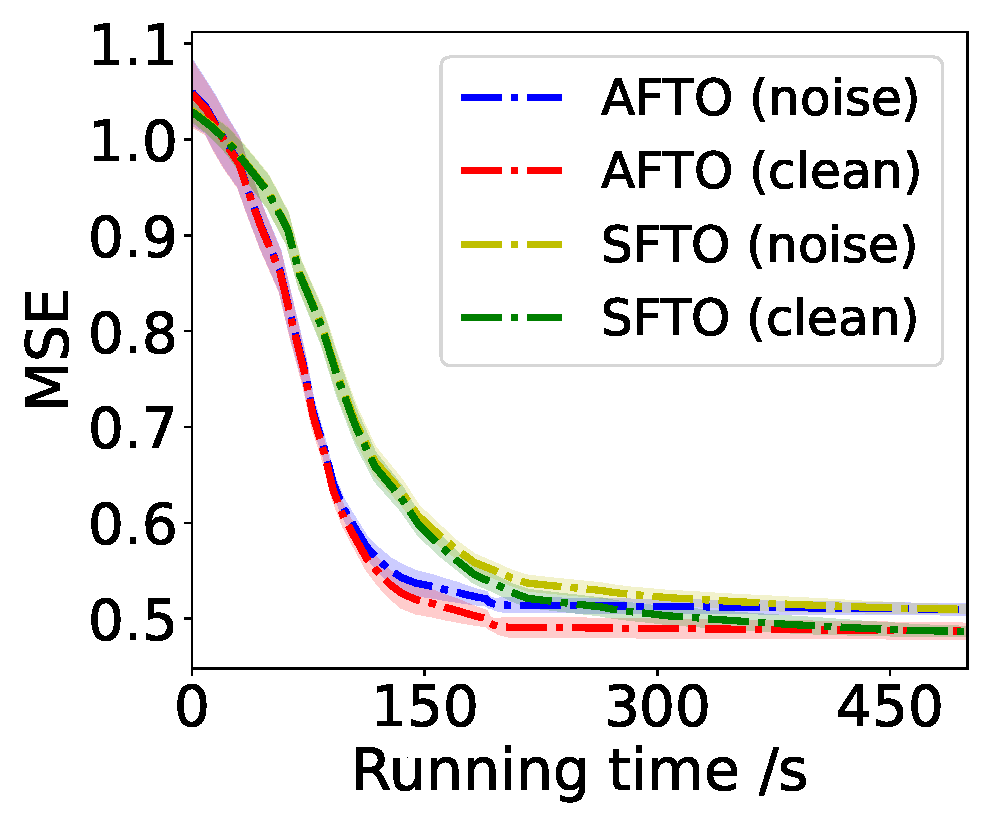
\includegraphics[scale=0.215]{dis-diabetes.pdf}
\end{minipage}}
\subfigure[Boston]
{\begin{minipage}{4.2cm}
\label{fig:dis-boston}   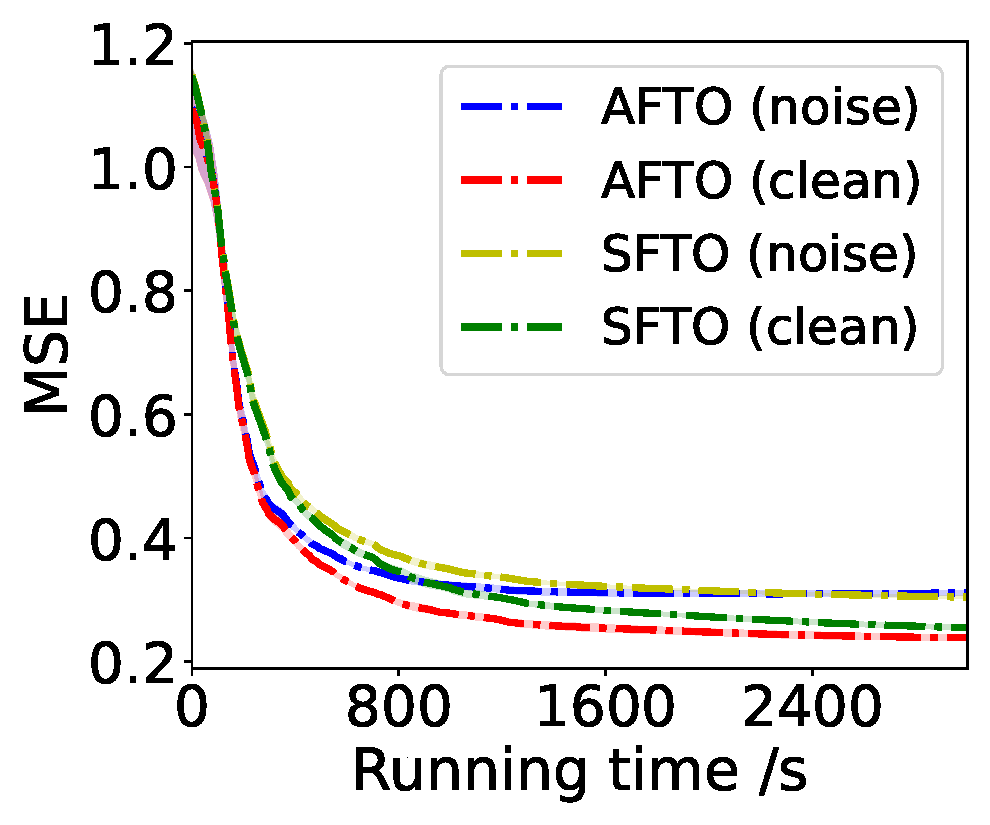
\includegraphics[scale=0.215]{dis-boston.pdf}
\end{minipage}}
\subfigure[Red-wine]
{\begin{minipage}{4.2cm}
\label{fig:dis-red}
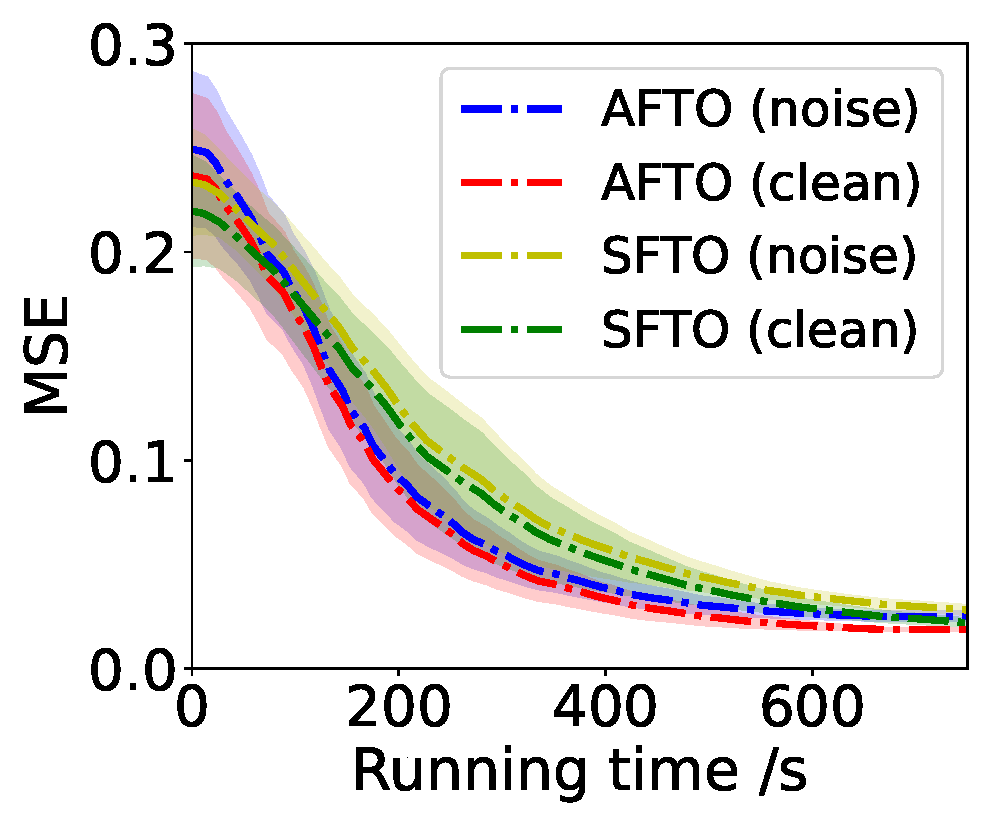
\includegraphics[scale=0.215]{dis-red.pdf}
\end{minipage}}
\subfigure[White-wine]
{\begin{minipage}{4.2cm}
\label{fig:dis-white}
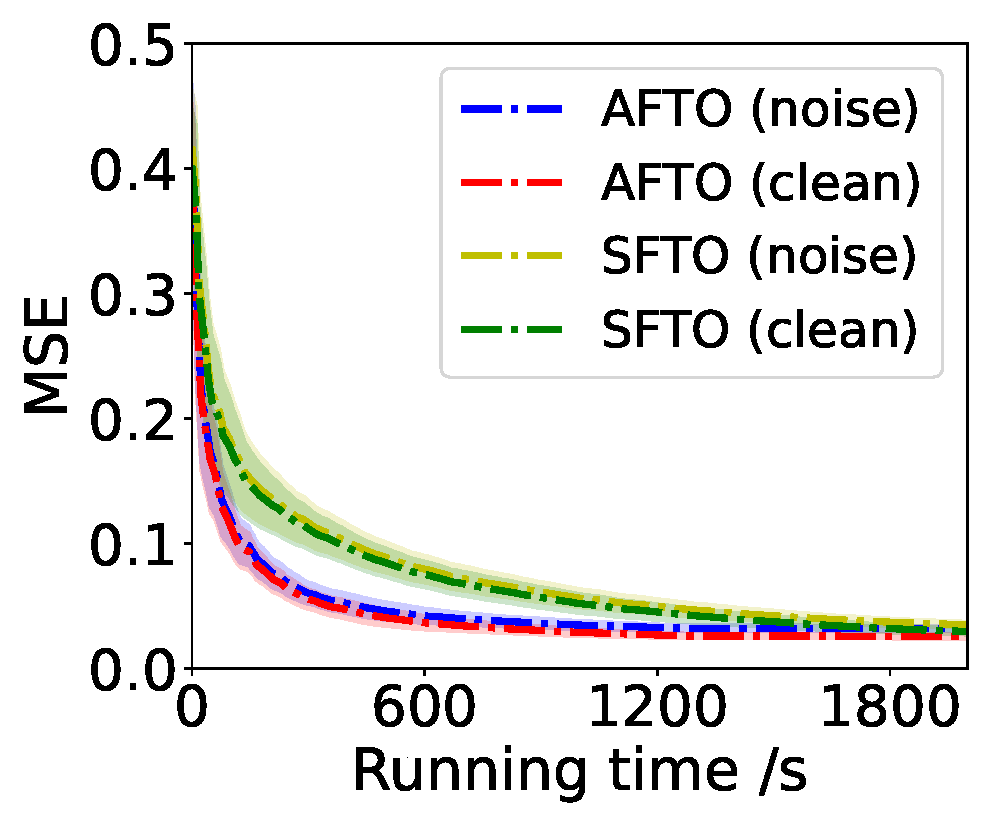
\includegraphics[scale=0.215]{dis-white.pdf}
\end{minipage}}
\caption{MSE of clean test data and test data with Gaussian noise
on (a) Diabetes, (b) Boston, (c) Red-wine quality, and (d) White-wine quality datasets. All experiments are repeated five times, and the shaded areas represent the standard deviation.} %  %
\label{fig:dis-hyper}
\end{figure*}

\begin{figure*}[t]
\centering
\subfigure[Test accuracy]
{\begin{minipage}{4.2cm}
\label{fig:dis-svhn-acc}
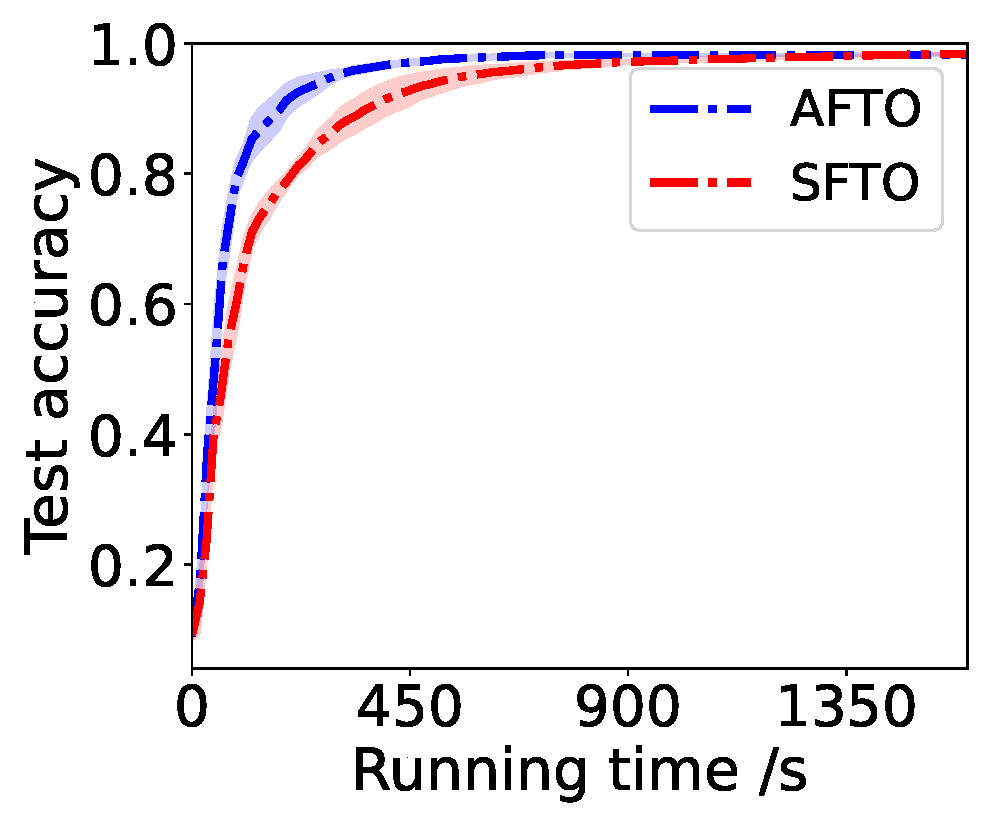
\includegraphics[scale=0.215]{dis-svhn-acc.pdf}
\end{minipage}}
\subfigure[Test loss]
{\begin{minipage}{4.2cm}
\label{fig:dis-svhn-loss}   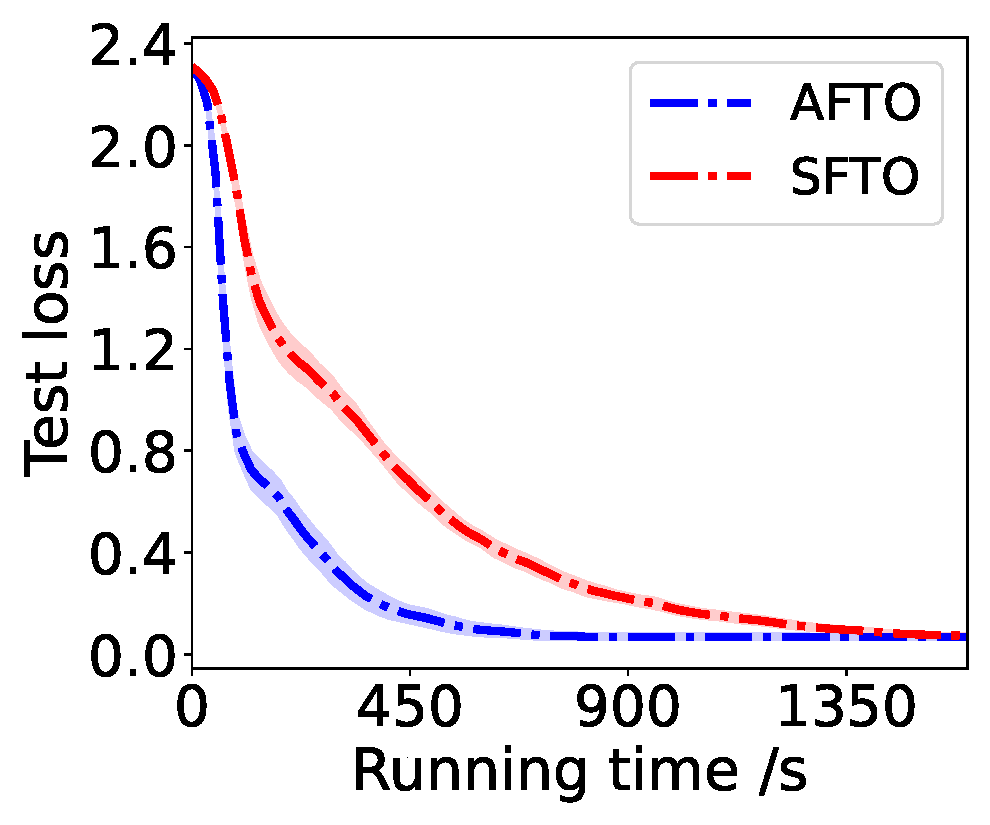
\includegraphics[scale=0.215]{dis-svhn-loss.pdf}
\end{minipage}}
\subfigure[Test accuracy]
{\begin{minipage}{4.2cm}
\label{fig:dis-pre-mnist-acc}
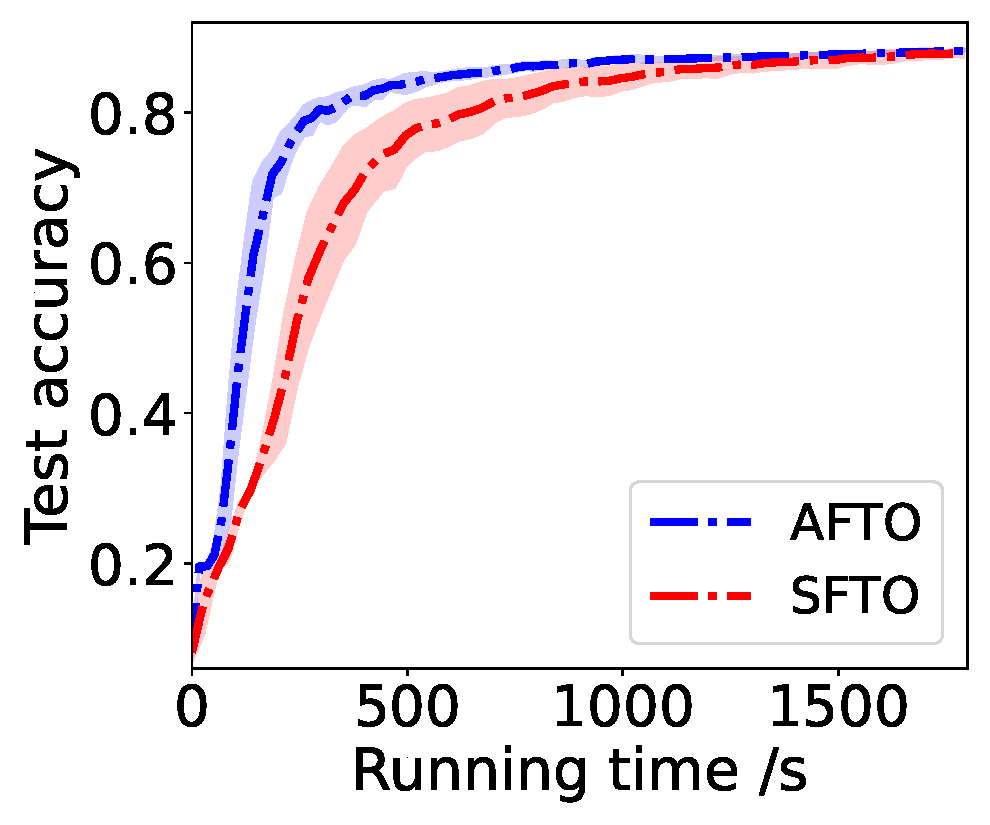
\includegraphics[scale=0.215]{dis-mnist-acc.pdf}
\end{minipage}}
\subfigure[Test loss]
{\begin{minipage}{4.2cm}
\label{fig:dis-pre-mnist-loss}
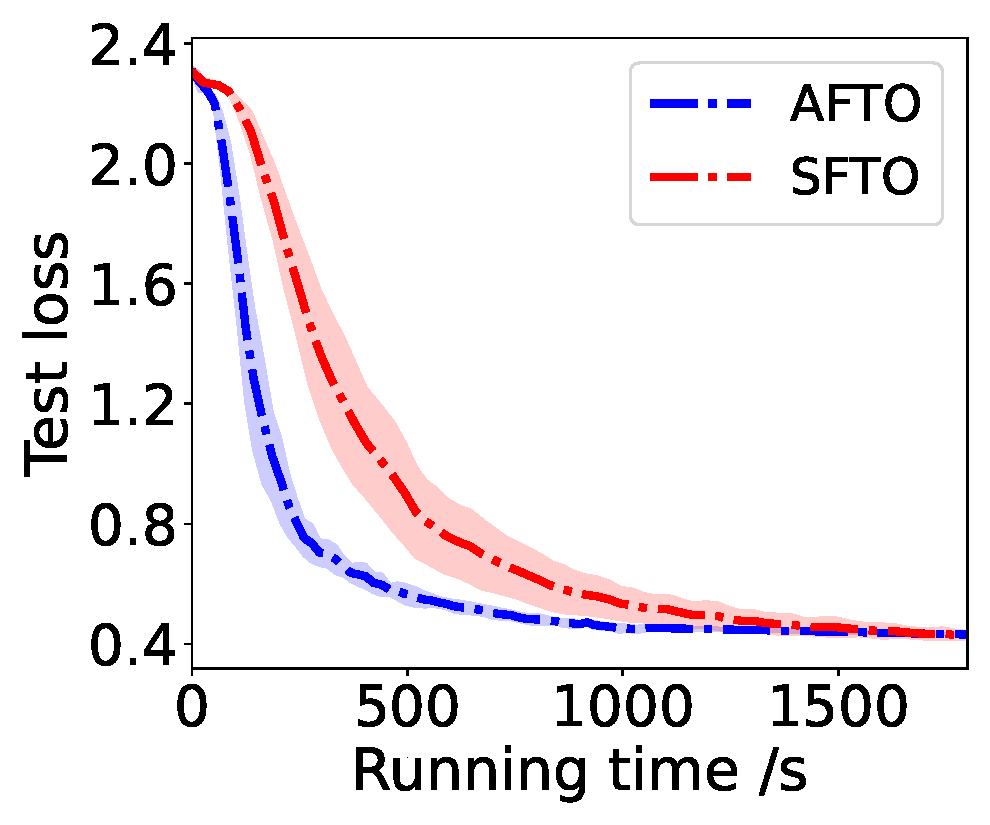
\includegraphics[scale=0.215]{dis-mnist-loss.pdf}
\end{minipage}}
\caption{(a) Test accuracy and (b) test loss vs running time when SVHN is utilized to pretrain the model. (c) Test accuracy and (d) test loss vs running time  when MNIST is utilized to pretrain the model. All experiments are repeated five times.} %  %
\label{fig:dis-domain}
\end{figure*}


\section{Experiment}

In the experiment, two distributed trilevel optimization tasks are employed to assess the performance of the proposed method. In the distributed robust hyperparameter optimization, experiments are carried out on the regression tasks  following \cite{sato2021gradient}, and in distributed domain adaptation for pretraining $\&$ finetuning, the multiple domain digits recognition task in \cite{qian2019robust,wang2021discriminative} is considered. The details of the experimental setting are summarized in Table \ref{tab:details_main} and Appendix H. More experimental results are reported in Appendix G. To further show the superior performance of the proposed method, experimental results of comparisons between the non-distributed version of the proposed method with existing state-of-the-art TLO methods \cite{sato2021gradient,choe2022betty} on three TLO tasks are shown in Appendix A in the supplementary material.



\subsection{Distributed Robust Hyperparameter Optimization}


The robust hyperparameter optimization \cite{sato2021gradient} aims to train a machine learning model that is robust against the noise in input data, which is inspired by bilevel hyperparameter optimization \cite{chen2022single} and adversarial training \cite{han2023fedal,zhang2022revisiting}. And we consider the following distributed robust hyperparameter optimization problem,
\begin{equation}
\begin{array}{l}
\mathop {\min }\sum\nolimits_{j} \frac{1}{|D^{\rm{val}}_j|}|| y^{\rm{val}}_j - f(X^{\rm{val}}_j;{\boldsymbol{w}})||^2 \;{\mathop{\rm s.t.}} \\

{\boldsymbol{p}} \!=\! \mathop {\arg \max } \limits_{{\boldsymbol{p}}'} \! \sum\nolimits_{j} (\! \frac{1}{{|D^{\rm{tr}}_j|}} ||y^{\rm{tr}}_j\! -\! f(X^{\rm{tr}}_j\! +\! {p_j'} ;{\boldsymbol{w}}) ||^2 \! -\! c||{p_j'} ||^2) \,{\mathop{\rm s.t.}}\\

{\boldsymbol{w}} \!=\! \mathop {\arg \min }\limits_{{\boldsymbol{w}}'}\!\sum\nolimits_{j}(\! \frac{1}{{|D^{\rm{tr}}_j|}} ||y^{\rm{tr}}_j\! -\! f(X^{\rm{tr}}_j \!+\! {p_j'} ;{\boldsymbol{w}}') ||^2  \!+\! e^{{\boldsymbol{\varphi }}} ||{\boldsymbol{w}}'||_{1*})  \\
{\mathop{\rm var.}} \qquad \quad {\boldsymbol{\varphi }} ,{\boldsymbol{p}},{\boldsymbol{w}},
\end{array}
\end{equation}
where ${\boldsymbol{\varphi }}$, ${\boldsymbol{w }}$ and ${\boldsymbol{p}}$ respectively denote the regularization parameter, model parameter, and adversarial noise,   ${\boldsymbol{p}}'=[p_1',\cdots,p_N']$, $N$ is the number of workers. $f$ denotes the output of a MLP, $c$ denotes the penalty for the adversarial noise, and $|| \cdot ||_{1*}$ is a  smoothed $l_1$-norm \cite{saheya2019neural}. $X^{\rm{val}}_j, y^{\rm{val}}_j, {|D^{\rm{val}}_j|}$, $X^{\rm{tr}}_j, y^{\rm{tr}}_j, {|D^{\rm{tr}}_j|}$ respectively denote the data, label and the number of data of the validation and training datasets on local worker $j$. Following \cite{sato2021gradient}, the experiments are carried out on the regression tasks with the following
datasets: Diabetes  \cite{dua2017uci}, Boston  \cite{harrison1978hedonic}, Red-wine and White-wine quality  \cite{cortez2009modeling} datasets. We summarize the experimental setting on each dataset in Table \ref{tab:details_main}. To show the performance of the proposed AFTO, we report the mean squared error (MSE) of clean test data and test data with Gaussian noise vs running time of the AFTO and SFTO (Synchronous Federated Trilevel Optimization) in Figure \ref{fig:dis-hyper}. It is seen that the proposed AFTO can effectively solve the TLO problem in a distributed manner and converges much faster than SFTO since the master can update its variables once it receives updates from a subset of workers instead of all workers in AFTO. Furthermore, we compare the proposed method with the state-of-the-art distributed bilevel optimization methods ADBO \cite{jiao2022asynchronous} and FEDNEST \cite{tarzanagh2022fednest}. It is shown in Table \ref{tab:ADBO-ATOP} that the proposed AFTO can achieve superior performance, which demonstrates the effectiveness of the proposed method.


\renewcommand\arraystretch{1.1}
\renewcommand\tabcolsep{10pt}
\begin{table}[t]
\centering
\renewcommand{\thetable}{\arabic{table}}
{
\begin{tabular}{l|c|c|c|c}
\toprule
& $N$     & $S$ & Stragglers & $\tau$ \\ \hline
Diabetes  & 4  & 3 & 1 & 10 \\
Boston & 4  & 3 & 1  & 10 \\
Red-wine & 4  & 3 & 1 & 10\\
White-wine & 6  & 4 &  1 & 10 \\
SVHN (finetune) & 4  & 3 & 1  & 5 \\
SVHN (pretrain) & 6  & 3 & 2  & 15\\
\bottomrule
\end{tabular}}
\caption{Experimental setting in distributed robust hyperparameter optimization and distributed
domain adaptation.}
\label{tab:details_main}
\end{table}

\renewcommand\arraystretch{1}
\renewcommand\tabcolsep{10pt}
\begin{table*}[t]
\centering
\renewcommand{\thetable}{\arabic{table}}
{
\begin{tabular}{l|c|c|c|c}
\toprule
Method   & Diabetes   & Boston  & Red-wine & White-wine   \\ \hline
FEDNEST  &  0.5293  0.0229 & 0.3509  0.0177 &  0.0339  0.0014  & 0.0268  0.0010  \\
ADBO  &  0.5284  0.0074 & 0.3243  0.0046 & 0.0336  0.0018 & 0.0277  0.0013  \\ \hline
\textbf{AFTO} & \textbf{0.5124}  \textbf{0.0068}  & \textbf{0.3130}  \textbf{0.0037} & \textbf{0.0321}  \textbf{0.0026} & \textbf{0.0248}  \textbf{0.0021} \\

\bottomrule
\end{tabular}}
\caption{MSE of test data with Gaussian noise, lower scores $\downarrow$ represent better performance which are shown in boldface.}
\label{tab:ADBO-ATOP}
\end{table*}



\subsection{Distributed Domain Adaptation}


Pretraining/finetuning paradigms are increasingly adopted recently in self-supervised
learning \cite{he2020momentum}.  In \cite{raghu2021meta}, a domain adaptation strategy is proposed, which combines data reweighting with a pretraining/finetuning framework to automatically
decrease/increase the weight of pretraining samples that cause negative/positive transfer, and can be formulated as trilevel optimization \cite{choe2022betty}. The corresponding distributed trilevel optimization problem is given as follows,
\begin{equation}
\begin{array}{l}
\; \mathop {\min } \sum\nolimits_{j} L_{FT,j}({\boldsymbol{\varphi }} ,{\boldsymbol{v}},{\boldsymbol{w}}) \;{\mathop{\rm s.t.}} \%removedVspace

\; {\boldsymbol{v}}\! =\! \mathop {\arg \min }\limits_{{\boldsymbol{v}}'} \sum\nolimits_{j} \left(L_{FT,j}({\boldsymbol{\varphi }} ,{\boldsymbol{v}}',{\boldsymbol{w}}) \!+\! \lambda ||{\boldsymbol{v}}' -{\boldsymbol{w}} ||^2  \right) \;{\mathop{\rm s.t.}} \\

\; {\boldsymbol{w}}\! =\! \mathop {\arg \min }\limits_{{\boldsymbol{w}}'} \!\sum\nolimits_{j} \! \frac{1}{\mathcal{D}_j}\!\sum\nolimits_{x_{i,j}\in\mathcal{D}_j}\! \mathcal{R}(x_{i,j}, {\boldsymbol{\varphi }})\!\cdot \! L_{PT,j}^i({\boldsymbol{\varphi }} ,{\boldsymbol{v}}',{\boldsymbol{w}}')  \\
\;  {\mathop{\rm var.}} \qquad \quad {\boldsymbol{\varphi }} ,{\boldsymbol{v}},{\boldsymbol{w}},
\end{array}
\end{equation}
where ${\boldsymbol{\varphi }}$, ${\boldsymbol{v}}$ and ${\boldsymbol{w}}$ respectively denote the parameters for pretraining, finetuning, and reweighting networks. $x_{i,j}$ and $L_{PT,j}^i$ represent the $i^{\rm{th}}$ pretraining sample and loss in worker $j$, $L_{FT,j}$ represents the finetuning loss in worker $j$. $\mathcal{R}(x_{i,j}, {\boldsymbol{\varphi }})$ denotes the importance of pretraining sample $x_{i,j}$, and $\lambda$ is the proximal regularization parameter. To evaluate the performance of the proposed method, the multiple domain digits recognition task in \cite{qian2019robust,wang2021discriminative} is considered.  There are two benchmark datasets for
this task: MNIST \cite{lecun1998gradient} and SVHN \cite{netzer2011reading}. In the experiments, we utilize the same image resize strategy as in \cite{qian2019robust} to make the format consistent, and LeNet-5 is used for all pretraining/finetuning/reweighting networks. We summarize the experimental setting in Table \ref{tab:details_main} and Appendix H. Following \cite{ji2021bilevel}, we utilize the test accuracy/test loss vs running time to evaluate the proposed AFTO. It is seen from Figure \ref{fig:dis-domain} that the proposed AFTO can effectively solve the distributed trilevel optimization problem and exhibits superior performance,  which achieves a faster convergence rate than SFTO with a maximum acceleration of approximately 80$\%$.


\section{Conclusion}

\vspace{-4.97mm}
\vspace{-1.66mm}
Existing trilevel learning works focus on the non-distributed setting which may lead to data privacy risks, and do not provide the non-asymptotic analysis. To this end, we propose an asynchronous federated trilevel optimization method for TLO problems. To our best knowledge, this work takes an initial step that aims to solve the TLO problems in an asynchronous federated manner. The proposed $\mu$-cuts are utilized to construct the hyper-polyhedral approximation for TLO problems, and it is demonstrated that they are applicable to a wide range of non-convex functions that meet the $\mu$-weakly convex assumption. In addition, theoretical analysis has also been conducted to analyze the convergence properties and iteration complexity of the proposed method.




\vspace{-2.24mm}  maxime quas, nulla delectus modi quisquam eveniet quos tenetur veniam sapiente.Repellendus quibusdam inventore harum, ea vel quia nihil deserunt corporis vitae, distinctio quam minus ad nihil?Commodi perferendis minima aspernatur suscipit rerum voluptatum culpa magnam asperiores consectetur, dignissimos molestias voluptates, numquam vero quia mollitia eius fugit quis totam recusandae earum officia, corrupti odit deserunt et quia harum, aspernatur repellat nostrum amet ullam sapiente.Unde doloremque vel asperiores veritatis ex expedita quibusdam exercitationem, eos cupiditate repudiandae corporis nulla mollitia consequuntur ipsa incidunt sunt, quo adipisci tempore fugit voluptatibus quam voluptatum consectetur iusto facere, hic rerum voluptates distinctio deserunt ex impedit ab expedita, recusandae laudantium enim sunt provident et?Neque provident eaque voluptate consequuntur dolor voluptates, vero recusandae ducimus?Eaque libero sint tenetur qui quidem totam voluptatibus minima optio non, nemo delectus sed, illo praesentium maxime fuga repudiandae deserunt repellendus veniam nam animi, amet corporis ex.Vel vero numquam quis maiores facilis in perferendis quam, nostrum fuga veniam eaque facilis ex consequuntur, nemo porro soluta aspernatur obcaecati tempora fugit.Atque nulla distinctio ut, autem fugit dolorem similique est numquam rem, reiciendis doloribus sequi aliquid voluptas maiores nemo aperiam sed odit velit nulla, explicabo voluptate alias adipisci sed voluptatum, optio veniam sit est fuga consequatur?Nisi omnis voluptates at asperiores perspiciatis voluptatibus placeat minima odio, cupiditate facilis molestias esse harum accusamus reiciendis sit, aliquam possimus pariatur eaque, sequi ipsum optio eius exercitationem odio aperiam minima.Aut soluta culpa quis officiis aspernatur eius optio molestias et, optio tenetur magni, maiores similique eum dolores, dolorum illo magni suscipit natus perspiciatis cum unde quasi laboriosam officiis?Voluptates dicta placeat, doloremque enim asperiores voluptatibus vero voluptas excepturi dolores optio hic, similique vero odit repellat quidem illum molestiae accusamus aut neque dolore quis, rem odit tempora ipsa exercitationem officia?Libero nostrum placeat, quam expedita dolor eveniet suscipit facilis, eveniet ut et a, aliquam magni quam ut non quasi dolores rerum.Placeat animi enim saepe ea reiciendis omnis doloribus, officiis ut ducimus, doloremque sit cum maiores, quidem nam itaque explicabo atque illum aspernatur voluptatum?Corrupti excepturi voluptatibus itaque, doloribus ad autem nihil?Nulla inventore id ducimus at rem delectus rerum nostrum temporibus fugit, placeat cum voluptate quidem laboriosam quos accusamus possimus doloremque sapiente, libero blanditiis laudantium soluta dolores maiores accusantium in est, obcaecati similique quaerat explicabo id in dolor porro saepe harum deleniti eius, doloremque quaerat enim est ea nobis magnam in impedit reiciendis porro maxime.Praesentium reprehenderit mollitia odio culpa ipsa magnam nesciunt, incidunt laudantium vitae vero pariatur, ex repudiandae vel debitis nisi voluptates soluta dignissimos quam repellat cum, corrupti voluptatem pariatur deserunt modi asperiores magnam libero, veniam similique minima impedit molestias atque et repellat deserunt quia enim?Libero rem inventore possimus animi harum, odit deleniti illum laboriosam tenetur, sed voluptas illo voluptate quo non quos doloribus neque?Earum officiis corporis repellendus vitae, animi repudiandae ipsa repellendus veritatis totam eaque distinctio blanditiis necessitatibus debitis maiores, autem natus doloribus odit voluptatem optio perspiciatis?Laborum aperiam aliquam itaque rerum accusantium quisquam animi sapiente dicta, quasi corrupti consectetur velit cupiditate nesciunt, soluta consequatur nesciunt blanditiis, obcaecati repellat iste ullam eos enim voluptate incidunt hic, expedita pariatur maiores tenetur consequatur ipsam possimus.Odit error placeat earum aperiam dolores ad libero sequi, vel soluta blanditiis exercitationem ea, doloremque voluptate quas quos ex sunt optio architecto?Dolores facilis obcaecati quos atque ad quaerat ab iusto maxime, architecto consequuntur hic illum, nulla consectetur velit, eligendi nobis perferendis, quos a amet fugiat.Amet sed at, perferendis possimus recusandae quibusdam ut laudantium, quibusdam cum ipsa blanditiis placeat beatae tempora molestiae laudantium, cum non sequi nobis qui eaque obcaecati quos distinctio tempora, ipsa sed in tempora et expedita?Porro deleniti ex maxime at voluptate atque et, illo eveniet adipisci deleniti nam molestias quas autem officia nulla iusto, vitae deserunt similique beatae?Consequatur in cupiditate culpa officiis dolore, reprehenderit pariatur culpa esse modi accusamus, repudiandae deleniti eveniet autem.Dolores quibusdam soluta, aperiam mollitia dolor repellat aliquid a rerum amet iste qui nesciunt, eveniet hic nihil consectetur modi libero, inventore reiciendis voluptas autem, aliquid vitae hic.Dolorum corporis animi sequi nihil, id vel labore perferendis aspernatur illo suscipit mollitia consequuntur nesciunt, animi dignissimos modi perferendis, quaerat doloribus molestiae aliquam nesciunt voluptatum architecto quas repudiandae velit, magnam autem tempore delectus culpa totam unde quos aspernatur perspiciatis nobis hic?\clearpage
\bibliography{aaai24}

\end{document}



